%%This is a very basic article template.
%%There is just one section and two subsections.
\documentclass{report}
\usepackage{authblk}
\usepackage{xcolor}
\usepackage{graphicx}
\usepackage{caption}
\usepackage{subcaption}
\usepackage{hyperref}
\usepackage{listings}
\usepackage{color}
\usepackage{url}
\usepackage[section]{placeins}

\makeatletter
\renewcommand{\@chapapp}{Module}
\makeatother

\setlength{\parskip}{1em}

\definecolor{dkgreen}{rgb}{0,0.6,0}
\definecolor{gray}{rgb}{0.5,0.5,0.5}
\definecolor{mauve}{rgb}{0.58,0,0.82}

\lstset{frame=tb,
  language=Java,
  aboveskip=3mm,
  belowskip=3mm,
  showstringspaces=false,
  columns=flexible,
  basicstyle={\small\ttfamily},
  numbers=none,
  numberstyle=\tiny\color{gray},
  keywordstyle=\color{blue},
  commentstyle=\color{dkgreen},
  stringstyle=\color{mauve},
  breaklines=true,
  breakatwhitespace=true,
  tabsize=3
}

\lstset{basicstyle=\ttfamily,
  showstringspaces=false,
  commentstyle=\color{red},
  keywordstyle=\color{blue}
}

\setlength{\parskip}{1em}

\begin{document}

\title{XSEDE Tutorial: High Performance Modeling and Simulation with Eclipse ICE}
\author{Jay Jay Billings}
\author{Andrew Bennett}
\author{Alex McCaskey}
\author{Robert Smith}
\author{Greg Watson}
\affil{Oak Ridge National Laboratory}

\maketitle{} 

\tableofcontents

\chapter{Overview and Installation}
\section{Overview}

\graphicspath{{../../installation/src/}}
\chapter{Paraview}

ICE features functionality for visualizing models using ParaView.

\section{Installation and Configuration}

ParaView use for ICE requires a Mac OS or Linux operating system, as ICE does
not currently support ParaView connections on Windows. You will also need an
installation of ParaView on your local machine. ParaView can be downloaded from
its \href{http://www.paraview.org/download/}{official website}. The ICE
development team recommends using the latest available version of ParaView,
currently 5.0 at the time of this writing. You will further need a custom
Python HTTP web server implementation, which can be downloaded from the
\href{http://eclipseice.ornl.gov/downloads/paraview/scripts/http_pvw_server.py}{Oak
Ridge website}.

\subsection{Configuring the ParaView Connection}

Once ParaView is running, ICE must be configured to connect to the server. This
is done through specifying a default connection in the ICE Preferences page.
This process only needs to be performed once. After initially creating the
connection, ICE will attempt to connect to ParaView on that port each time it is
launched.

To set the connection, select Window $\rightarrow$ Preferences\ldots in ICE's
menu bar. (On Mac OS X, Preferences\ldots is located under ICE instead of
Windows.) Select Visualization $\rightarrow$ ParaView in the tree on the left
side of the Preferences window.

\begin{center}
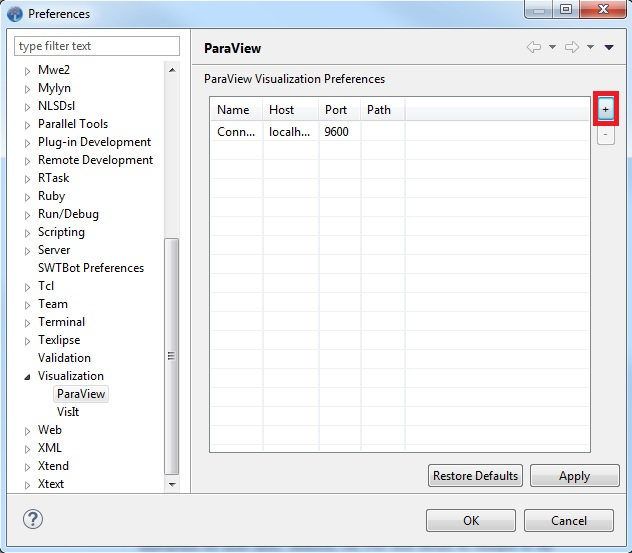
\includegraphics[width=12cm]{images/paraviewpreferencepage_ice}
\end{center}

Press the button with a ''+" symbol in the upper right (highlighted in the image
above) to add a new row to the table. Click on cells in the new row to edit
their values. 

\textbf{Name:} The connection's name. The default value will be fine.

\textbf{Host:} The hostname for the machine that will run ParaView. Use "localhost" if the machine running ICE will also be used to run ParaView.

\textbf{Port:} The port number on which the ParaView server will run. The default value will be fine, but if you change it, it must different from the Visualizer Port.

\textbf{Path:} The path to your ParaView installation. 

On Linux, the path will end with the top level folder into which ParaView was unzipped. For example, if you have a folder named ParaView on your desktop that contains the bin, doc, lib, and share folders, then your path would be /home/username/Desktop/ParaView. 

On Mac, the path will end with the folder containing your ParaView.app. For example, if you have installed ParaView to your Applications folder, the path will simply be /Applications

\textbf{Server Script Path:} The full path to the http_pvw_server.py file, ending with the folder containing it. For example if the file is on your desktop, the path might be /home/username/Desktop.

\textbf{Visualizer Port:} The port number for the ParaView web visualizer. The default value will be fine, but if you change it, then it must be different from the port number you provide for Port.

\textbf{Remote OS:} The operating system of the remote machine on which ParaView will be launched. If you want to launch ParaView on your local machine, ignore this cell. Otherwise, specify either "Linux" or "OSx".

\textbf{Remote ParaView Version Number:} The version of ParaView you are using. This may be ignored unless you are launching a remote ParaView session on a Linux machine. You can check your installation's version number by looking inside the top level \textbf{lib} folder. It will contain a folder named paraview- followed by the version number.

Once finished editing the cells in the new row, press Apply, then OK. ICE will
then launch the ParaView server and connect to it. If you are connecting to a remote machine, you will be prompted for permission to make the remote connection and asked for a password.

\section{Opening a ParaView File} 

To open a ParaView Plot Editor, a file that uses this editor must first be
placed in the Project Explorer. This view lists files imported into ICE. To
access the Project Explorer, use the the menu bar at the top of the window and
navigate to Window $\rightarrow$ Show View $\rightarrow$ Project Explorer.
Depending on the active Eclipse perspective, opening this view may require
selecting Other\ldots and finding the Project Explorer in the dialog under the
General category in the tree.

By default, the Project Explorer should automatically import the
ICEFiles/default and ICEFiles/itemDB folders. If it does not, or if you want to
import a different folder into ICE, right click in the Project Explorer and
select Import\ldots from the context menu. Then, select General $\rightarrow$
File System from the tree, and press the Next button. Select directories and/or
files to import into the Project Explorer, and enter which folder they should
be imported into, as shown below.

\begin{center}
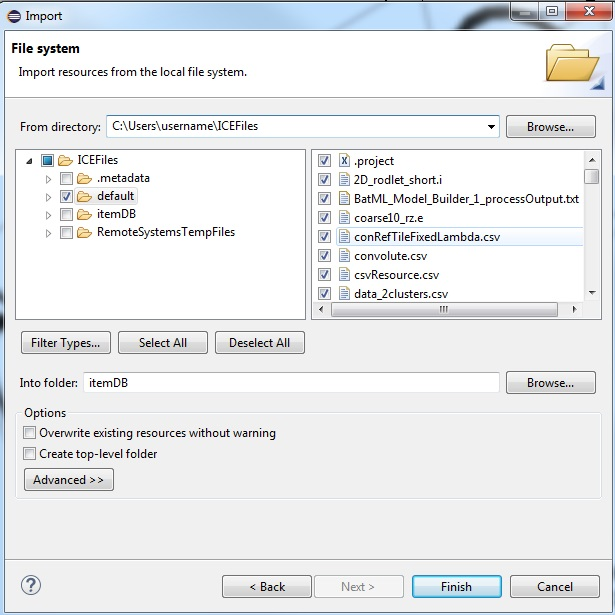
\includegraphics[width=12cm]{images/ImportFileDialog}
\end{center}

Once a file is in the Project Explorer, simply double click on it to open it in
ParaView. Local ParaView connections can only open local files, while remote ParaView connections can only open files on the remote host.

\subsection{Using ParaView}

\subsubsection{Camera Controls}

The Plot Editor allows the user to rotate the model by clicking and dragging
inside the display area or adjust the zoom by scrolling the mouse wheel.

\begin{center}
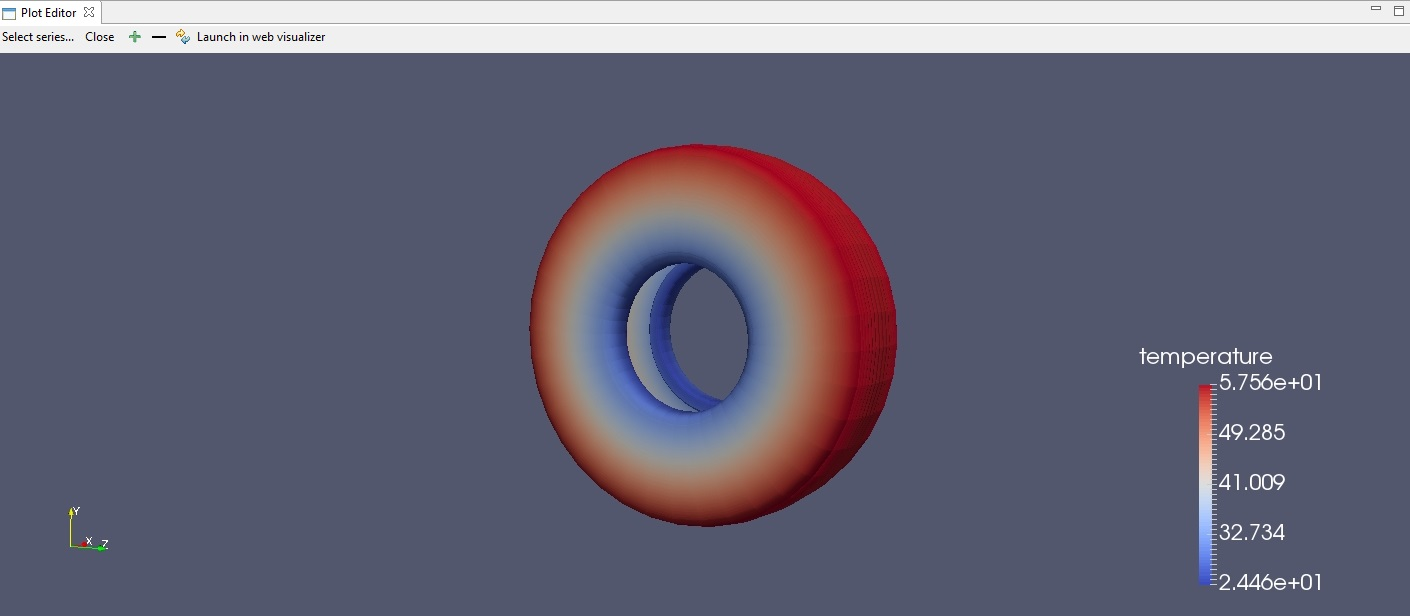
\includegraphics[width=12cm]{images/ParaViewPlotEditor}
\end{center}

The buttons in the upper left can also be used to manipulate the camera. The green plus sign will zoom in, while the black minus sign will zoom out. The green circular arrow button will reset the camera to its default position.

\subsubsection{Selecting the Plot}

Pressing the Select Series\ldots button will open a dialog which lists the
various plots in the opened file. Simply select one and click OK to open it. 

\begin{center}
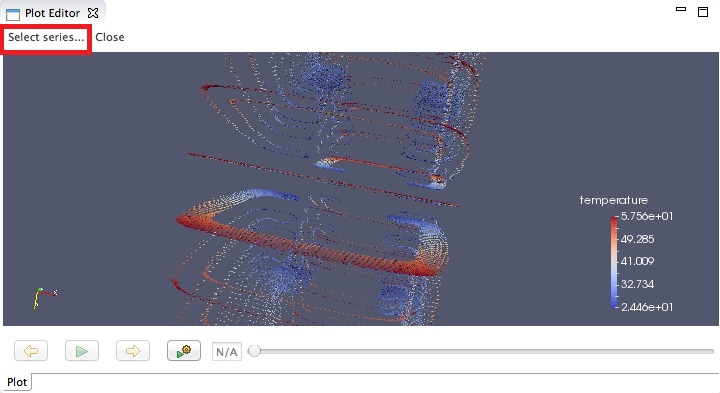
\includegraphics[width=12cm]{images/ParaViewPlotEditorSelectSeriesButton}
\end{center}

\subsubsection{Setting the Plot Representation} 

ParaView is capable of displaying plots in several different representations,
such as points or surfaces. To switch between plot type, right click inside the Plot
Editor's display area and select one of the listed options under the
Representation category in the context menu.

\begin{center}
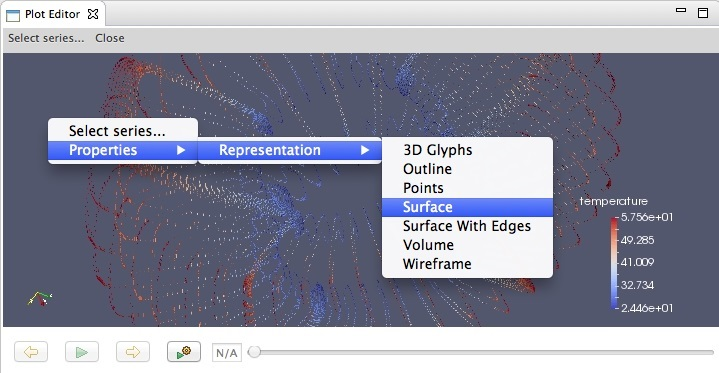
\includegraphics[width=12cm]{images/ParaViewRepresentationDropDown}
\end{center}

\subsubsection{Animation and Time Data}

The Plot Editor features a time slider widget at the bottom of the screen. 

\begin{center}
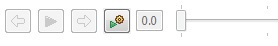
\includegraphics[width=12cm]{images/TimeSliderWidget}
\end{center}

The controls, in order of left to right, are:

1) Return to the previous time step.

2) Automatically play the plot as an animation by displaying the time steps
sequentially. 

3) Advance to the next time step. 

4) Opens an options menu that allows the user to set the playback speed, toggle
whether the animation should loop when it reaches the end, and set the plot to
the first or last time step.

5) A display for the current time step. It can be edited to set the plot to an
arbitrary time step. 

6) A slider that shows the current time step's position on the timeline. The
slider can be dragged around the timeline, setting the plot's time step
accordingly.

\section{Accessing a ParaView Web Server}

It is also possible to access the full ParaView web viewer application inside of
ICE. This allows for full access to all the web viewer's features.

\subsection{Accessing the Visualizer}

First, you must open a Plot Editor as described above.

\begin{center}
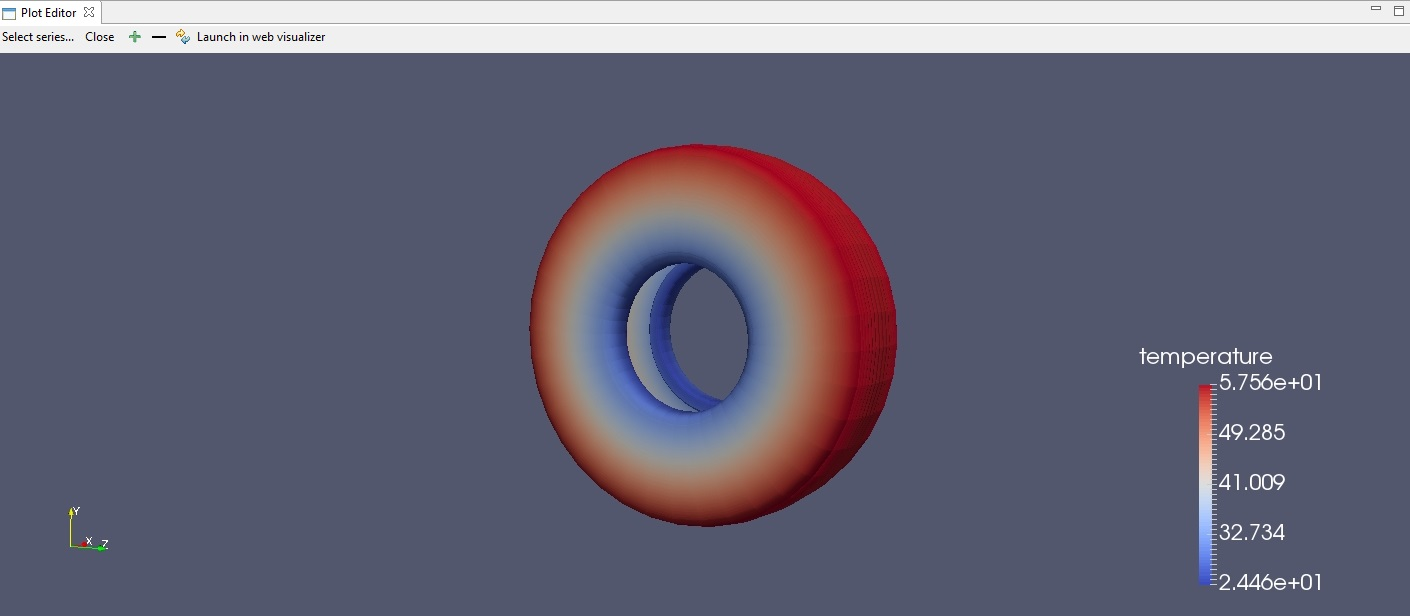
\includegraphics[width=12cm]{images/ParaViewPlotEditor}
\end{center}

Press the "Open in Web Visualizer" button in the top left to launch the web visualizer server and automatically open an internal web browser to view it.

\subsection{Using the Visualizer}

In order to load a data file, click the Show File List button as seen below.

\begin{center}
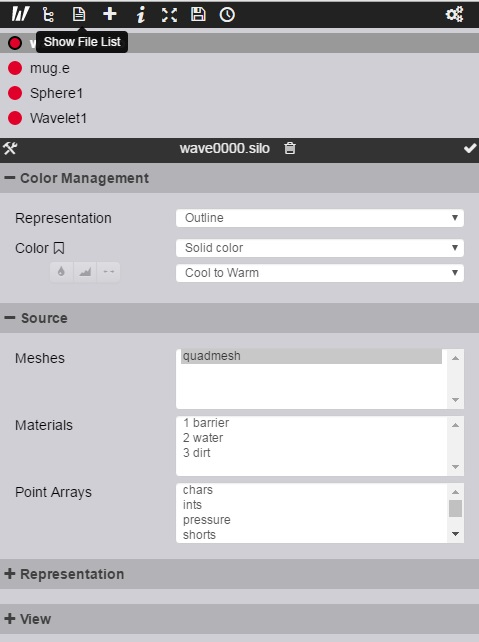
\includegraphics[width=12cm]{images/ParaViewVisualizer}
\end{center}

This will place the contents of the data directory into the side bar. For sessions, the data directory will be your ICE workspace. For a remote connection, this will be the folder containing the remote file you are visualizing. You may then double click on a file to load it into the model. 

You can click and drag the mouse to rotate the camera and right click followed
by dragging up or down to zoom. A full description of the visualizer's features
is beyond the scope of this tutorial, but see the official documentation
\href{http://www.paraview.org/ParaView3/Doc/Nightly/www/js-doc/index.html#!/guide/web_visualizer}{here}.

\chapter{Creating and Using an Application Dashboard}
\graphicspath{{../../newItemGeneration/src/}}
\section{Creating an ICE Item} 

This tutorial will teach you how to
create your own ICE Items via the built-in tools within ICE.  To demonstrate
these tools, we will walk through the development of a dashboard for the
FERN code, a fast, efficient nuclear reaction network solver. 

After creating a new ICE Item plugin project, we will demonstrate how to
provide a few lines of code to create an editor for
input files for FERN. After that we will show how a small amount of code can be
used to create a job launcher that is customized to execute FERN locally. We
will also show how to launch FERN remotely.

\subsection{Creating the Project}

\begin{figure}[h]
\centering
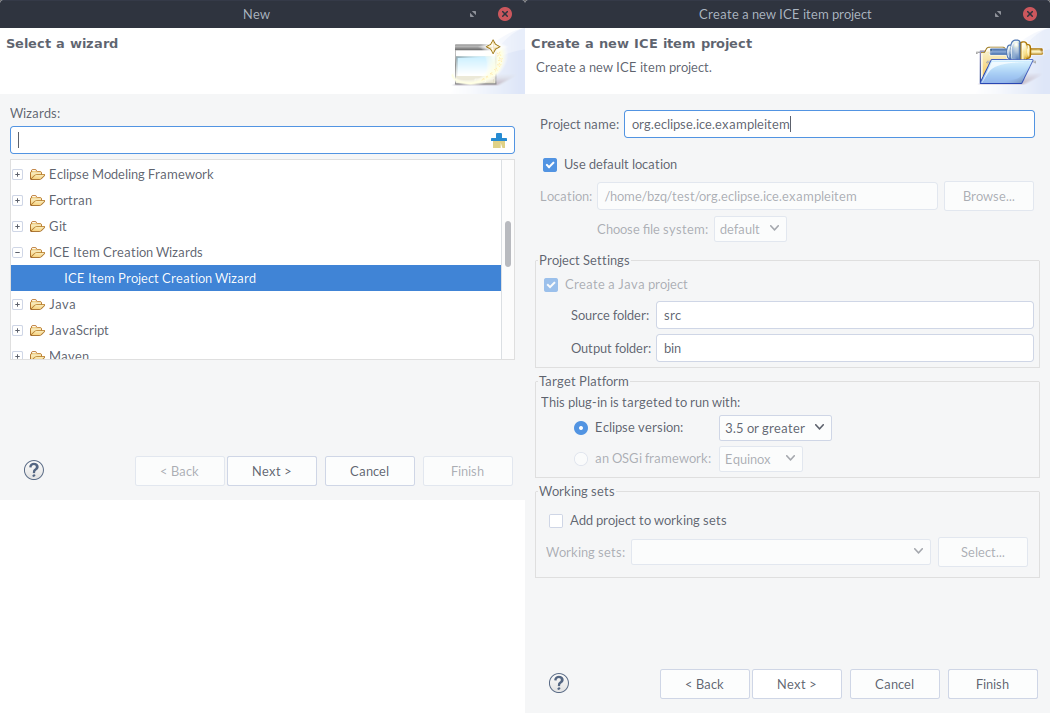
\includegraphics[width=\textwidth]{figures/comb12.png}
\label{fig:comb12}
\end{figure}

To create a new ICE Item project, navigate to \texttt{File $\rightarrow$ New
$\rightarrow$ Other}. Open the \texttt{ICE Item Creation Wizards} folder and 
select \texttt{ICE Item Creation Wizard}. You will be met with a standard new
project wizard page, in which you can name your project.  We will call ours
\texttt{org.eclipse.ice.fern}. Once you have named your project click the \texttt{Next>} button.
\begin{center} 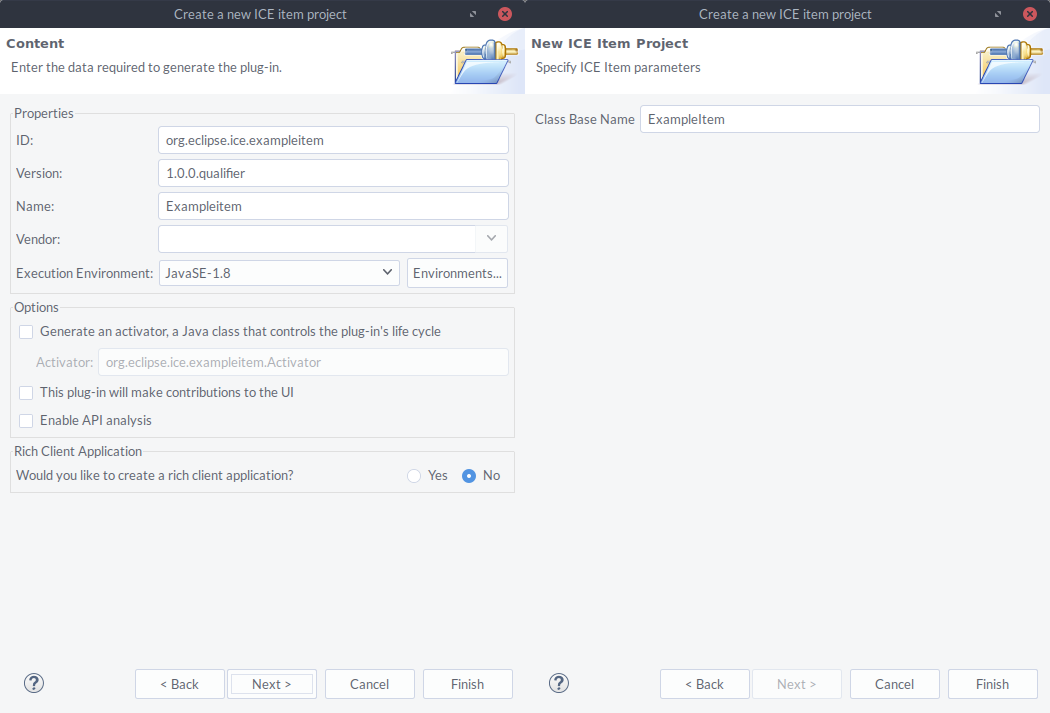
\includegraphics[width=\textwidth]{figures/comb23} \end{center}

The next dialog page enables you to customize the plugin-specific
portions of the project. For this tutorial, we will leave all the settings at
their defaults. Simply click \texttt{Next>} to move to the next page. 

On this page you need to tell the wizard what you want to use as a base
name for your item classes. We will call this one \texttt{Fern}. Then, we will
specify some information about how the item will handle input data.  FERN uses
the INI file format to specify data, so we will tell our item to use the built-in
functionality for INI files.  To do this select \texttt{INI} from the \texttt{File Format} dropdown.  

When you have entered all of the required information you can
click the \texttt{Finish} button to generate your new ICE Item plugin project.
When the project has finished generating you should be able to explore the code
that has been created.  Within the source directory there will be two packages,
each containing two Java classes:

\begin{itemize} 
    \item \texttt{org.eclipse.ice.fern.launcher} 
    \begin{itemize}
        \item \texttt{FernLauncher.java} 
        \item \texttt{FernLauncherBuilder.java}
    \end{itemize} 
    \item \texttt{org.eclipse.ice.fern.model} 
    \begin{itemize} 
        \item \texttt{FernModel.java} 
        \item \texttt{FernModelBuilder.java}
    \end{itemize} 
\end{itemize}

To add functionality to the project we need to edit
the \texttt{FernLauncher} and \texttt{FernModel} classes.

\subsection{Adding Functionality to the New Items}

\subsubsection{The Fern Model}

The \texttt{FernModel} will be responsible for creating and
validating input parameters for FERN, in the form of a new FERN input file.  In
order to make the generated code run there are several pieces of information that need to be changed.  First, we
will need to set up the basic Item idenfification information. This information
is set in the setupItemInfo() method. Modify the outputName to match the
following (or something of your choosing, with a .ini file extenstion).

\begin{lstlisting}[language=Java]
outputName = "fern_config.ini";
\end{lstlisting}

The String for the \emph{setName} method will serve as the display name
for this Item, so set it as \texttt{Fern Model}.
As for the String for \emph{setDescription}, this will also be used on the UI
for the Item, so provide some text like the following: \texttt{This Item constructs input files
for the FERN reaction network solver}. The export string will serve as the name
of the action that the user can select to write the provided data to file. Set
it to something like: \texttt{Export to INI}. You should now have a method that
looks like this:

\begin{lstlisting}[language=Java]
@Override
protected void setupItemInfo() {
	setName("Fern Model");
	setDescription("This Item constructs " +
	    "input files for the FERN reaction " +
	    "network solver"); 
	outputName = "fern_output.ini";   
	exportString = "Export to INI";
	allowedActions.add(0, exportString);
	ioFormat = "INI";
	defaultFileName = "";
}
\end{lstlisting}

The \emph{allowedActions.add()} line ensures that the export string is provided
to ICE as an allowed action, and displayed in the Item Process drop down.

With the identification information configured properly we can begin to
implement the Form for this FERN Model. This is done in the \emph{setupForm()}
method.
The generator has begun the process of implementing this method by instantiating
a Form for you to use, getting a reference to the IOService (which provides
IReader/IWriter realizations), and providing a commented out example of how to
fill out an ICE Form.

For this FERN input model, we want to add the following sections with data
entries: a network section with 
numSpecies, numReactions, numReactionGroups, massTol, fluxFrac, networkFile,
rateFile data entries, an initialConditions section with T9, startTime, endTime,
initialTimeStep, and density, and an output section with a single popFile
data entry.
To achieve this for this Item, we will need to add three
\texttt{DataComponents}, one for the network section, another for the
initialConditions section, and a final one for the outputs section. To each of
those DataComponents we will add appropriate IEntry instances for each of the data entries we have.

Add the following to your setupForm() method: 

\begin{lstlisting}[language=Java]

    // Create the network section
    DataComponent networkComp = new DataComponent();
    networkComp.setName("network");
    networkComp.setDescription("The parameters needed " +
        "to describe the nuclear " +
    	"reaction network"); 
    networkComp.setId(1);
    
    // Create the IEntries we need for this DataComponent
    StringEntry numSpecies = new StringEntry();
    numSpecies.setName("numSpecies");
    numSpecies.setDescription("The number of species to consider");
    numSpecies.setDefaultValue("16");
    
    StringEntry numReactions = new StringEntry();
    numReactions.setName("numReactions");
    numReactions.setDescription("The number of reactions to consider");
    numReactions.setDefaultValue("48");
    
    StringEntry numReactionGrps = new StringEntry();
    numReactionGrps.setName("numReactionsGroups");
    numReactionGrps.setDescription("The number of reaction " + 
    	"groups to consider"); 
    numReactionGrps.setDefaultValue("19");

    StringEntry massTol = new StringEntry();
    massTol.setName("massTol");
    massTol.setDescription("The mass tolerance to consider");
    massTol.setDefaultValue("1e-7");
    
    StringEntry fluxFrac = new StringEntry();
    fluxFrac.setName("fluxFrac");
    fluxFrac.setDescription("The flux fraction to consider");
    fluxFrac.setDefaultValue(".01");
    
    FileEntry networkFile = new FileEntry(".inp");
    networkFile.setProject(project);
    networkFile.setName("networkFile");
    networkFile.setDescription("The network file for this problem");
    
    FileEntry rateFile = new FileEntry(".data");
    rateFile.setProject(project);
    rateFile.setName("rateFile");
    rateFile.setDescription("The rate file for this problem");
    
    networkComp.addEntry(numSpecies);
    networkComp.addEntry(numReactions);
    networkComp.addEntry(numReactionGrps); 
    networkComp.addEntry(massTol);
    networkComp.addEntry(fluxFrac);
    networkComp.addEntry(networkFile);
    networkComp.addEntry(rateFile);
    
    // Create the initial conditions section
    DataComponent initConditionsComp = new DataComponent();
    initConditionsComp.setName("initialConditions");
    initConditionsComp.setId(2);
    initConditionsComp.setDescription("The parameters " +
    	"needed to describe the	initial " + 
    	"conditions for the problem");
    
    StringEntry t9 = new StringEntry();
    t9.setName("T9");
    t9.setDescription("The temperature in Kelvin x 10^9");
    t9.setDefaultValue("7.0");

    StringEntry startTime = new StringEntry();
    startTime.setName("startTime");
    startTime.setDescription("The start time for the simulation.");
    startTime.setDefaultValue("1e-20");

    StringEntry endTime = new StringEntry();
    endTime.setName("endTime");
    endTime.setDescription("The end time for the simulation");
    endTime.setDefaultValue("1e-3");

    StringEntry initialTimeStep = new StringEntry();
    initialTimeStep.setName("initialTimeStep");
    initialTimeStep.setDescription("The initial time step " + 
    	"for the simulation."); 
    initialTimeStep.setDefaultValue("1.2345e-22");

    StringEntry density = new StringEntry();
    density.setName("density");
    density.setDescription("The initial density.");
    density.setDefaultValue("1e8");
    
    initConditionsComp.addEntry(t9);
    initConditionsComp.addEntry(startTime);
    initConditionsComp.addEntry(endTime);
    initConditionsComp.addEntry(initialTimeStep);
    initConditionsComp.addEntry(density);
    
    // Create the outputs section
    DataComponent outputComp = new DataComponent();
    outputComp.setName("output");
    outputComp.setDescription("The parameters needed to output data.");
    outputComp.setId(3);
    
    StringEntry popFile = new StringEntry();
    popFile.setName("popFile");
    popFile.setDescription("The name of the output populations file");
    popFile.setDefaultValue("popFile.csv");
    
    outputComp.addEntry(popFile);
    
    // Add the components to the Form
    form.addComponent(networkComp);    
    form.addComponent(initConditionsComp);
    form.addComponent(outputComp);
    
\end{lstlisting}

Now we have a Form constructed for a typical FERN execution. 

The default generated implementation of the process method is sufficient to be
able to create new FERN INI input files. 

\subsubsection{Fern Launcher}
A FERN launcher handles the actual execution of the FERN application. The
generator creates the FernLauncher as a subclass of ICE's JobLauncher, which
provides a large array of features and functionality. As a subclass of
JobLauncher, the FernLauncher enables users to execute FERN locally or remotely.
To do so, we just need to add a small amount of
code that customizes the ICE job launching capabilities for FERN. 

The first bit of code to add to the FernLauncher specifies the name of the
actual Fern executable. In the setupItemInfo() method, set the execCommand to
the following: 
\begin{lstlisting}[language=Java]
execCommand = "${installDir}fern-exec";
\end{lstlisting}
This tells ICE that the FERN executable is called \texttt{fern-exec}, and to
set the overall execution command to it's install path plus the executable name.
The installDir flag will tell ICE to insert the user-specified executable
location (provided through the graphical form editor') into the execCommand,
with a trailing OS-specific path separator. This install directory is
specified through the Hosts Table on the editory. 

We also need to inform the JobLauncher what other files are involved in this
execution. To do that, the JobLauncher provides an addInputType() method. Add
the following to setupForm():
\begin{lstlisting}[language=Java]
addInputType("Network File", "networkFile", 
			"Network File Description", ".inp");
addInputType("Rate File", "rateFile", "
			Rate File Description", ".data");
\end{lstlisting}

And that should be it.
The generator has taken care of everything else for us.
We are now ready to launch ICE with our FERN plugin, and use the FERN Items we
have just created.

\section{Using the Application Dashboard} 

In order to use the functionality you've added to ICE, it is necessary to start
a new \textit{instance} of ICE, called the \textit{runtime} instance. This will
be a completely new copy of ICE that has your new plugins actived. This new
instance is how you and your users will typically interact with your
application. Once you are statisfied with the functionality you have added, you
can create a new \texttt{runtime application} that can be deployed to users.
Creating runtime applications is beyond the scope of this tutorial.

\subsection{Launching a New ICE Instance}

From the \texttt{Developer} top-level menu, select \texttt{ICE $\rightarrow$ Launch New Instance}. This will display a
dialog asking you which new plugins you'd like to include as part of the new ICE instance. 
\begin{center} 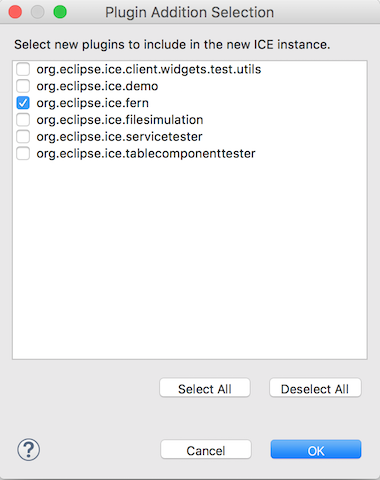
\includegraphics{figures/pluginDialog}
\end{center}
Select \texttt{org.eclipse.ice.fern} (or whatever name you chose for your
plugins) and click \texttt{OK}.
This will create and launch a new instance of ICE that includes your custom
plugins.

\subsection{Importing a Project}

This section will show you how to import an existing application project into
ICE so that you can use it with the dashboard you have just created. The steps
are as follows:

\begin{enumerate}
\item With a new ICE instance open, close the Welcome view if necessary
\item Go to \texttt{Package Explorer} view, right click and select \texttt{New
$\rightarrow$ Synchronized C/C++ Project}

\begin{center} 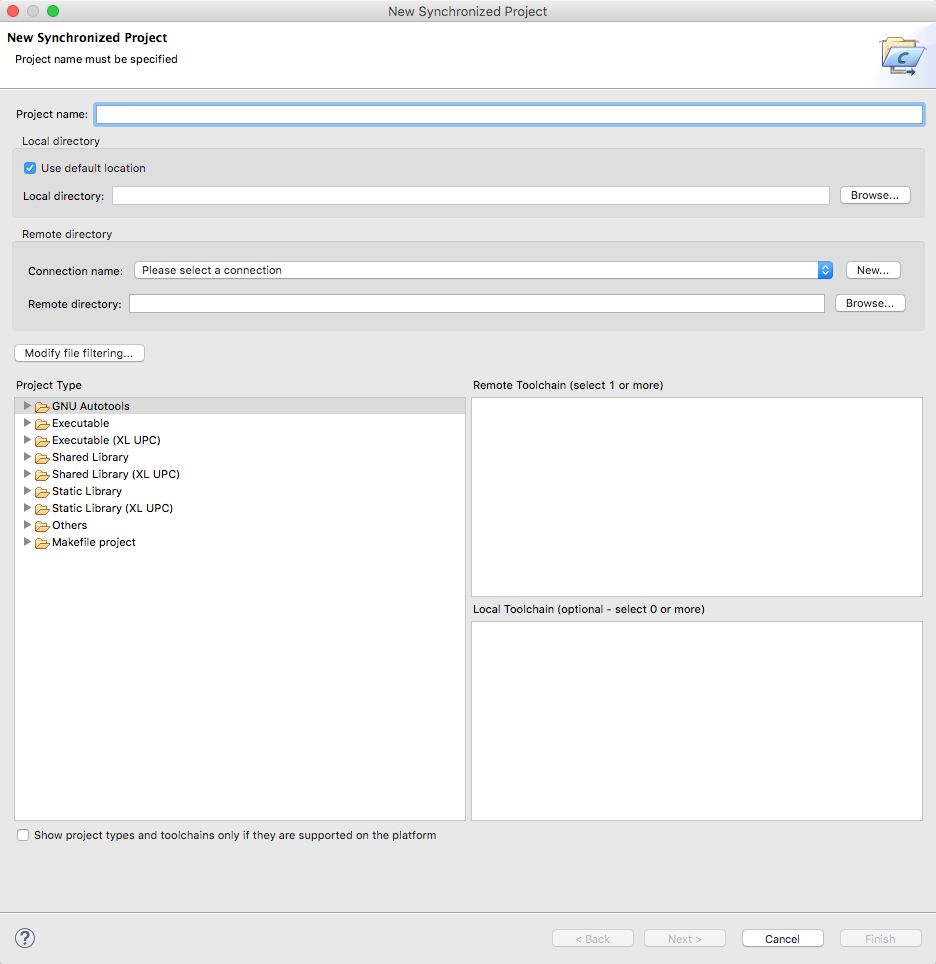
\includegraphics[width=\textwidth]{figures/newSyncWizard}
\end{center}

\item Enter \texttt{fern} for the \texttt{Project name:}
\item Click the \texttt{New\ldots} button next to the \texttt{Please select a
connection} dropdown

\begin{center} 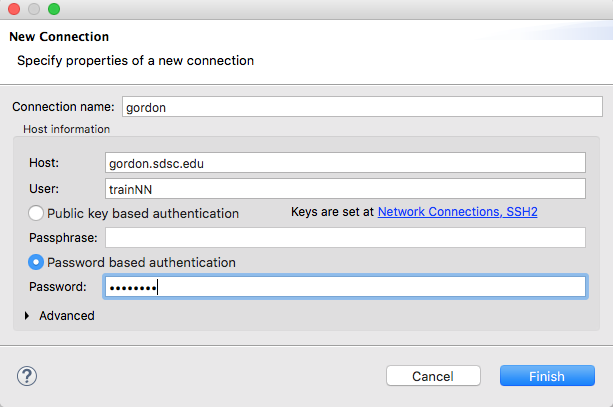
\includegraphics[width=300]{figures/newConnectionDialog}
\end{center}

\item Enter \texttt{gordon} for the \texttt{Connection name}
\item Enter \texttt{gordon.sdsc.edu} for the \texttt{Host}
\item Enter your training username for the \texttt{User}
\item Click on the \texttt{Password based authentication} button
\item Enter the training account password
\item Click \texttt{Finish}
\item Click on the \texttt{Browse\ldots} button
\item Select \texttt{fern} from the directory browser and press \texttt{OK}
\item Under \texttt{Makefile project} choose \texttt{Empty Project}
\item Click \texttt{Finish}
\end{enumerate}

At this point you should see a \texttt{fern} project in the \texttt{Project
Explorer} view. After a few moments it should complete the synchronization
and when you open the project you will see it contains a variety of files.

\subsection{Building a Project (Optional)}

We have provided a pre-built executable in the \texttt{build} subdirectory for
the purposes of this tutorial. However if you wish to build Fern yourself, you
can proceed as follows:

\begin{enumerate}
  \item Right click on the project and select \texttt{Properties}
  \item Click on the \texttt{C/C++ Build} entry
  \item Append \texttt{build} to the end of the \texttt{Build directory} entry
  \item Click \texttt{OK}
  \item Click on the hammer icon in the toolbar
\end{enumerate}

\subsection{Creating an Input File For Your Application}

To use ICE to create an input file, you first need to instantiate the
\texttt{FernModel} you created previously. To do this, right click on the
\texttt{fern} project (the location you want the files to be located), then
choose \texttt{New $\rightarrow$ Other},  select the
\texttt{Create Item Wizard}, then click on \texttt{Next>}.
\begin{center} 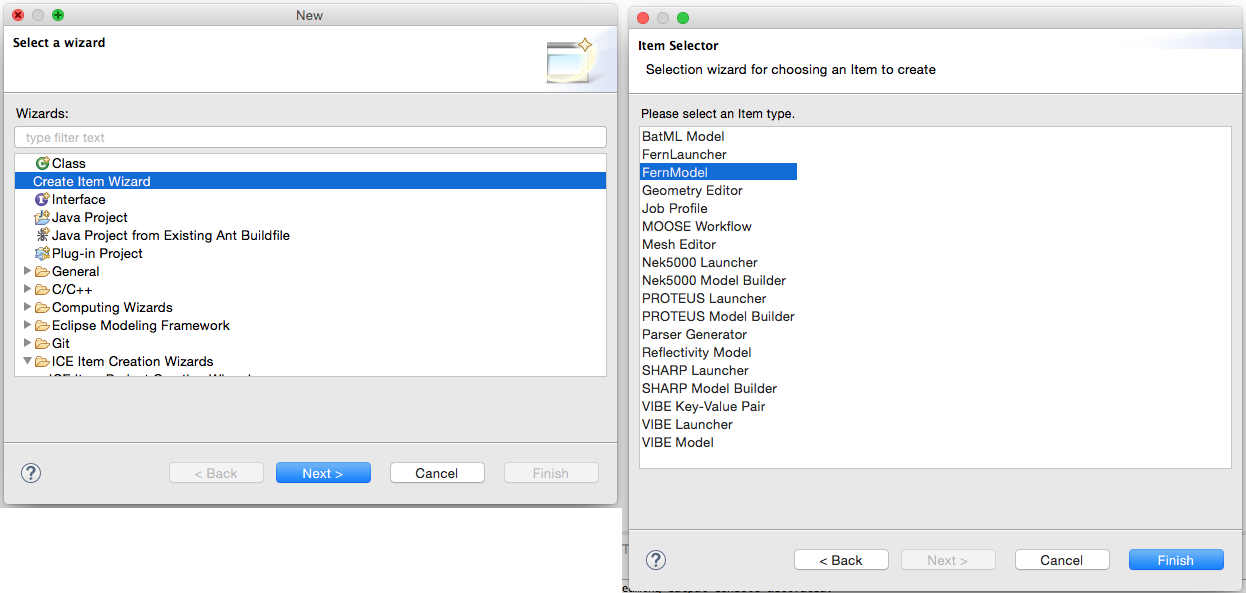
\includegraphics[width=\textwidth]{figures/creatingFernModelItem}
\end{center}
Selecting the \texttt{FernModel} Item, then click \texttt{Finish}, and you will
be presented with the view in the figure below. 
\begin{center} 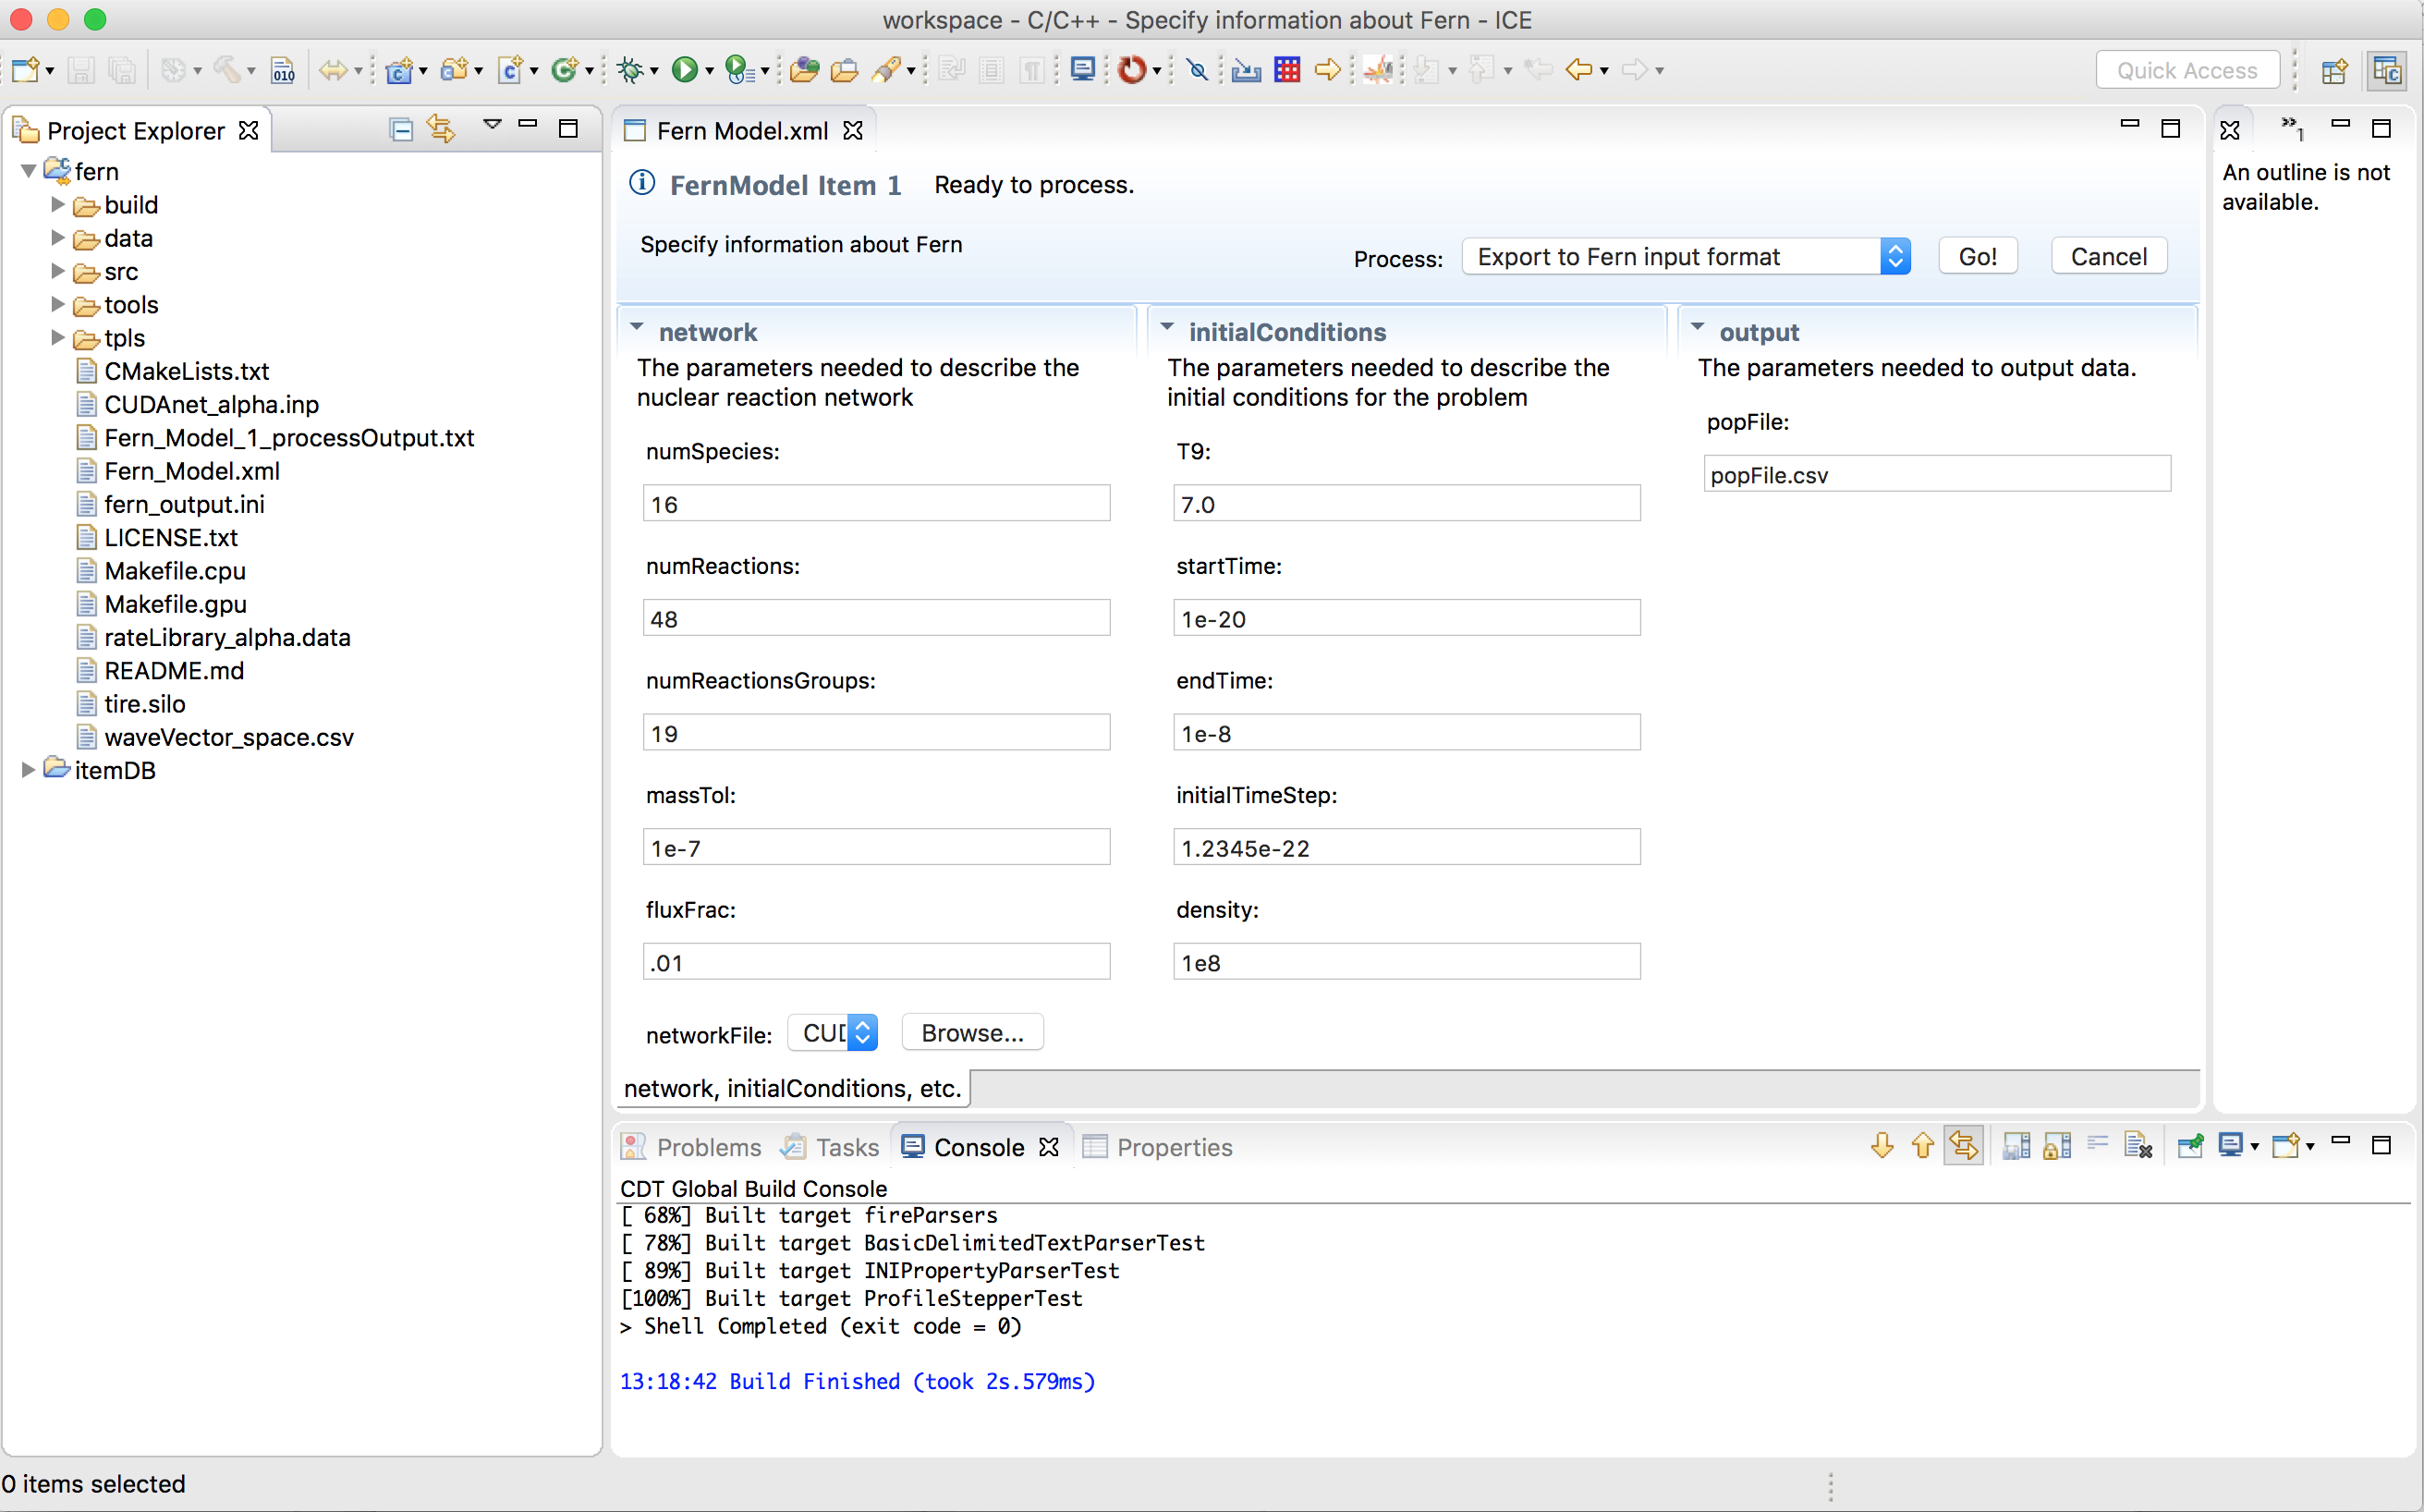
\includegraphics[width=\textwidth]{figures/fernmodelItem}
\end{center}
Here you can modify the various defaults with the values you would like for a
given Fern simulation. Once done, simply save the Item and click Go on the
Export to INI Process. This will execute the process of creating a new INI Fern
input file for use with the Fern Launcher. You can check the result by opening
the fern\_output.ini file, as shown below. 
\begin{center} 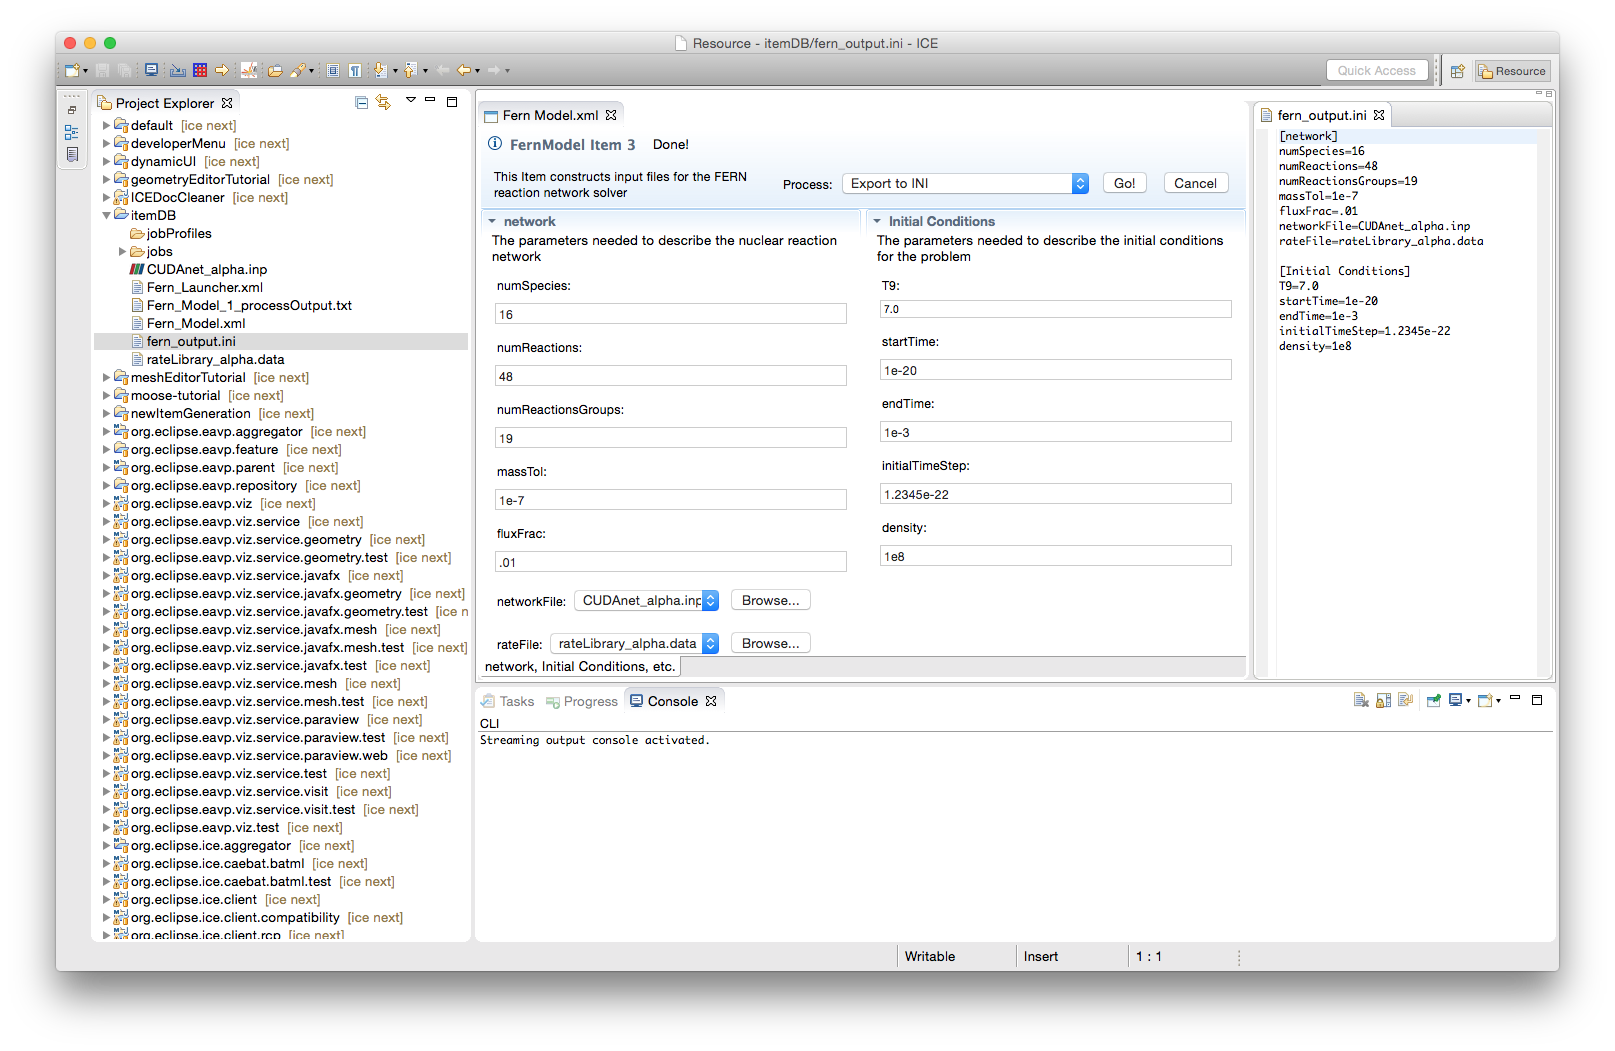
\includegraphics[width=\textwidth]{figures/result}
\end{center}

\subsection{Creating a Local Launcher}

Now you can similarly create a new Fern Launcher. Note that as Fern is not
installed locally, we will not acutally launch the program using this method.

After creating the Launcher,
you should see a view like below. 
\begin{center} 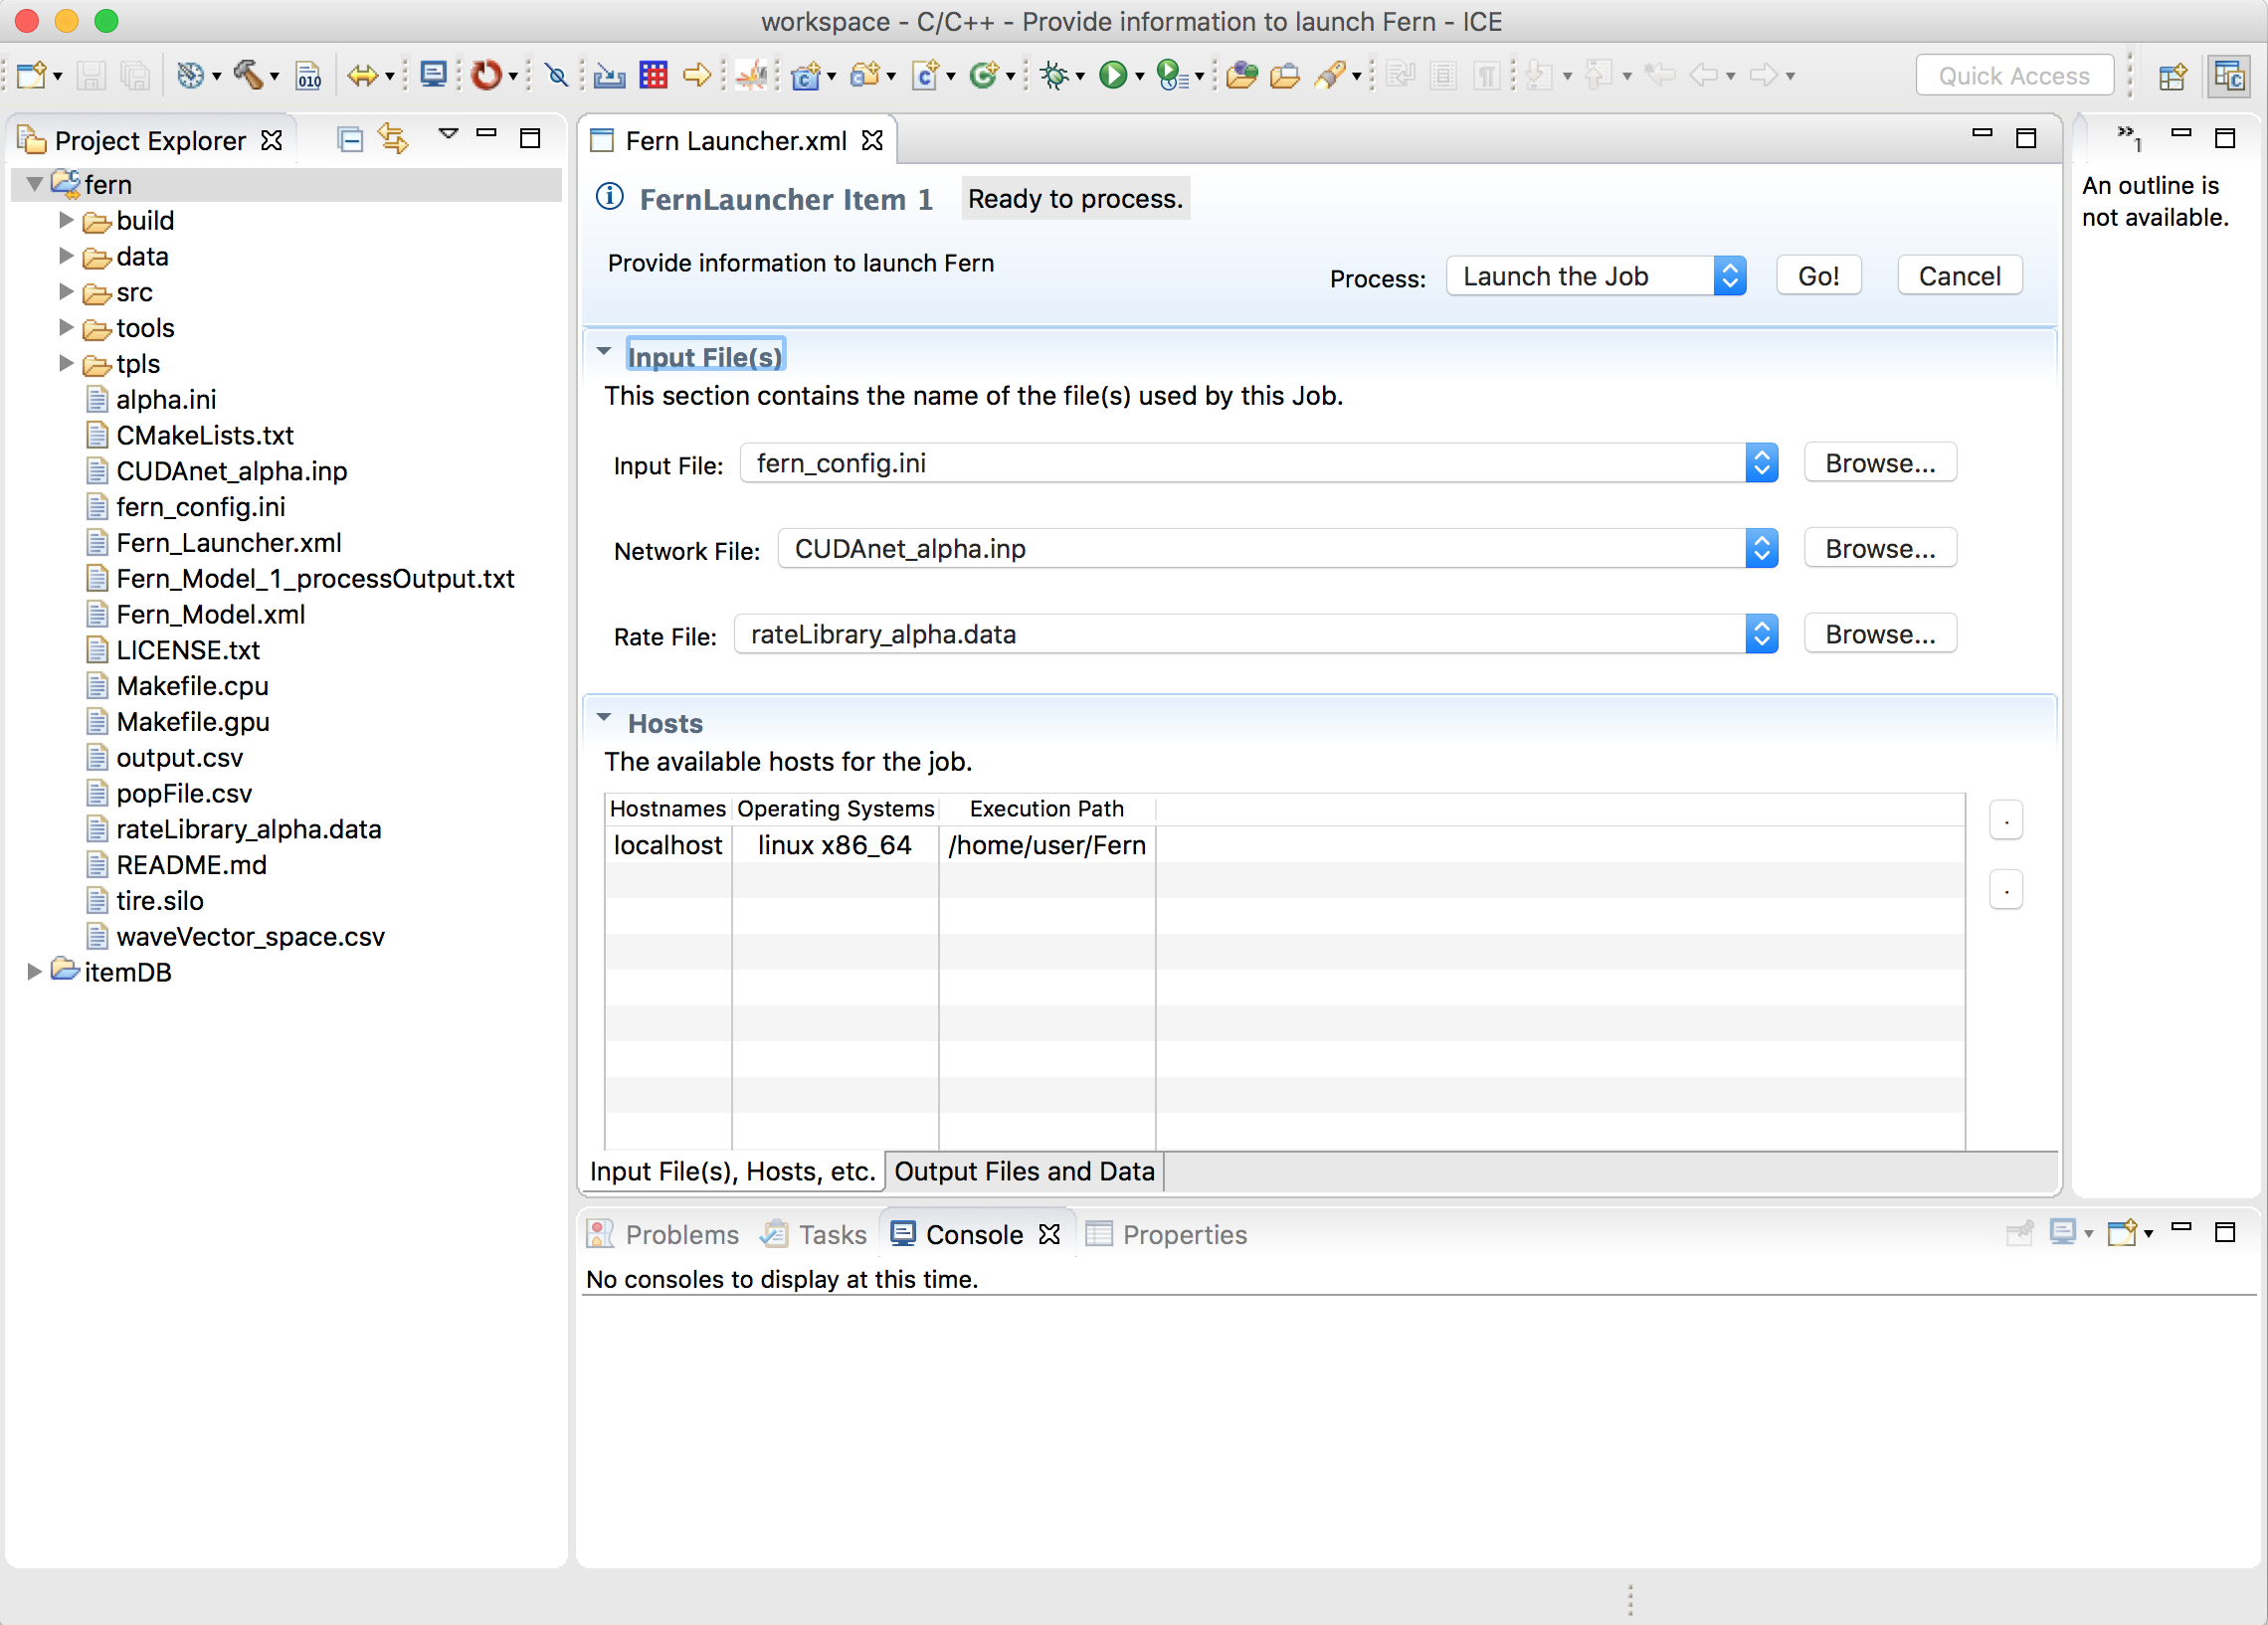
\includegraphics[width=\textwidth]{figures/launcher}
\end{center}
To configure a launch, simply set the correct
input file, along with its dependent network and rate files. 

At this point, if you had Fern built on your local machine, or if you had it
built on some remote host, you could configure that in the Hosts table. ICE
would then execute Fern based on that input. 

After the execution you should see the results in the Console, as shown below.
\begin{center} 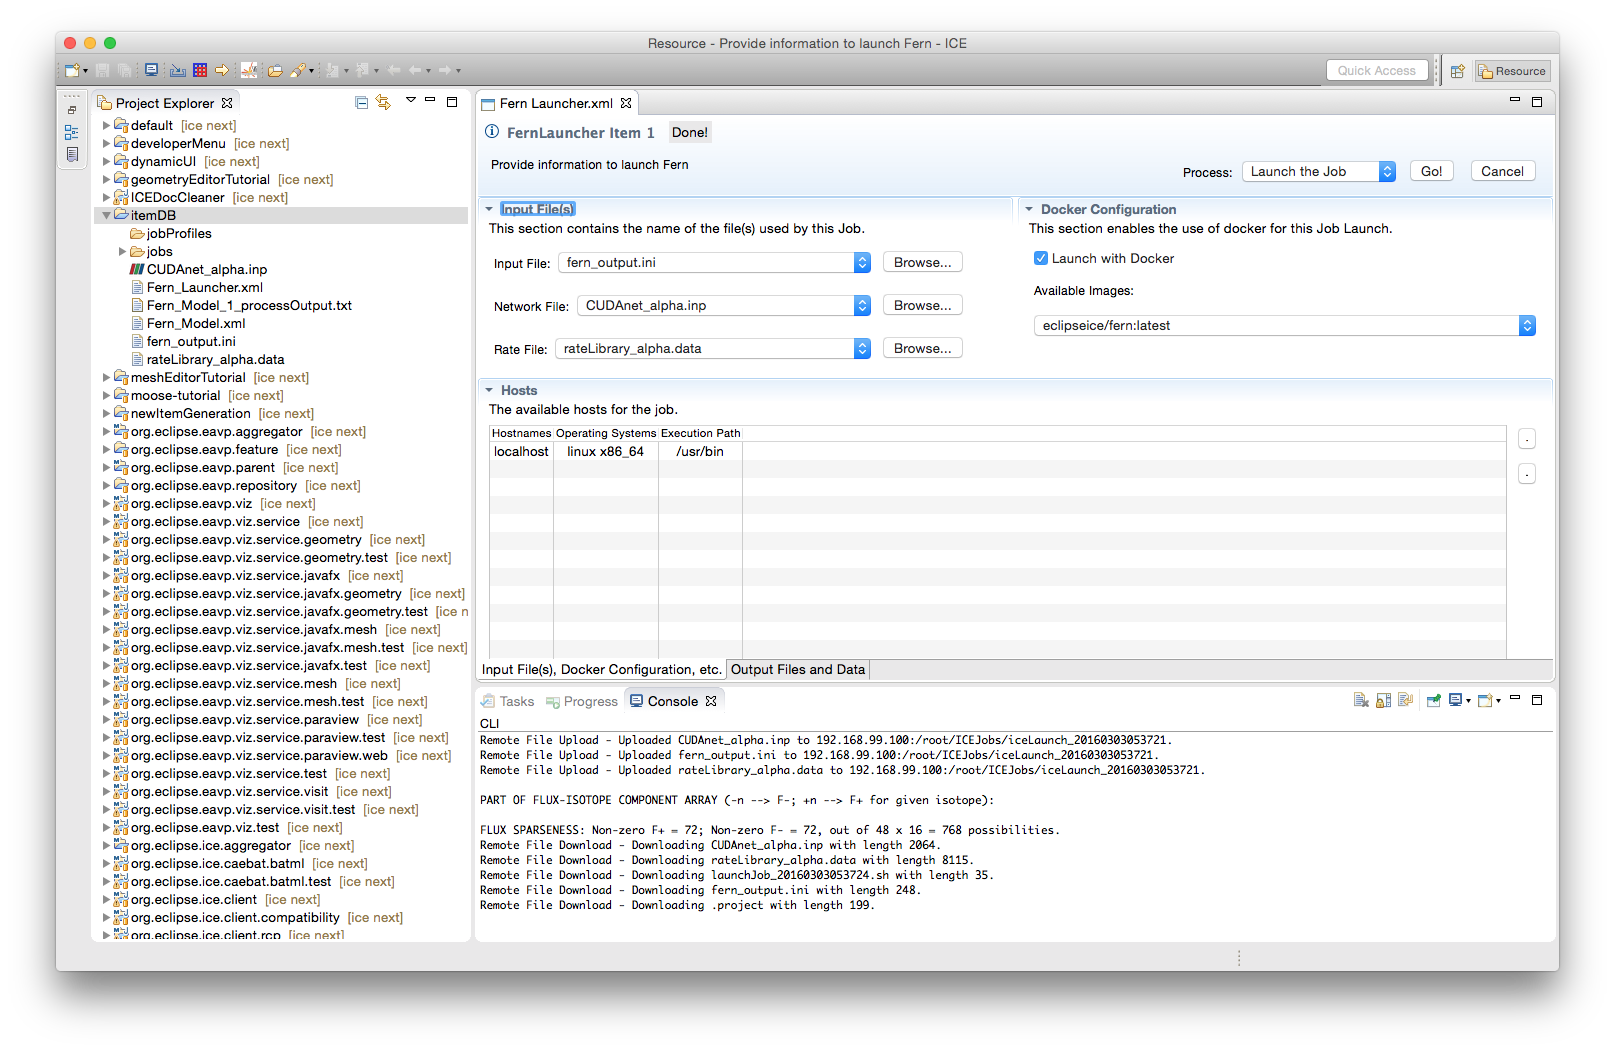
\includegraphics[width=\textwidth]{figures/launcherResult}
\end{center}
The execution should have produced a CSV file with the computed populations. You
can double-click that file to view them graphically in the ICE Plot Editor. 

\subsection{Creating a Remote Launcher}

Launching Fern remotely will involve creating a Parallel launch configuration.
This procedure is not yet integrated with the ICE launcher, but will be
available in the next release of ICE.

A Parallel launch configuration for your application is created as follows:

\begin{enumerate}
  \item Select the \texttt{Run $\rightarrow$ Run Configurations\ldots} menu
  \item Click on the \texttt{Parallel Application} entry, then click the
  \texttt{New} button
  \item From the \texttt{Target System Configuration} dropdown, select
  \textttt{Generic Torque Batch}
  \item From the \texttt{Please select a connection}, choose the \texttt{gordon}
  connection you created earlier
  \item Click \texttt{Yes} when asked if you would like to run a command on the
  remote system (optionally check the box to not ask again)
  \item After a few seconds, you should see the job submission form
  \item Select \texttt{normal} for the queue
  \item Switch to the \texttt{Application} tab
  \item If the project field doesn't contain anything, click \texttt{Browse} and
  choose the \texttt{fern} project
  \item Click \texttt{Browse} next to the \texttt{Application program} field,
  open the \texttt{build} directory, select \texttt{fern-exec}, then click
  \texttt{OK}
  \item Switch to the \texttt{Arguments} tab and enter the name of the
  outputfile you chose in the \texttt{FernModel} file
  \item Uncheck \texttt{Use default working directory}
  \item Click \texttt{Run} to submit the job 
\end{enumerate}

During the job submission, you will be asked if you would like to switch to the
\texttt{System Monitoring} perspecive. Click \texttt{Yes} to see this feature.
The image belows shows a typical instance of this perspective in action.

Click on the \texttt{Inactive Jobs} view and scroll to the bottom. You should
see a job from your username that is either submitted or completed. When the job
is completed, you can switch back to the \texttt{C/C++ Perspective}.

In the \texttt{Project Explorer} view, click on the \textit{synchronize}
button. Then open the \texttt{build} folder and you should see the resulting
CSV file. You can double click on this file to launch the CSV viewer.



\chapter{Adding Visualization to your Application}
\graphicspath{{../../resourceComponents/src/}}
\section{Creating an ICE Item} 

This tutorial will teach you how to
create your own ICE Items via the built-in tools within ICE.  To demonstrate
these tools, we will walk through the development of a dashboard for the
FERN code, a fast, efficient nuclear reaction network solver. 

After creating a new ICE Item plugin project, we will demonstrate how to
provide a few lines of code to create an editor for
input files for FERN. After that we will show how a small amount of code can be
used to create a job launcher that is customized to execute FERN locally. We
will also show how to launch FERN remotely.

\subsection{Creating the Project}

\begin{figure}[h]
\centering
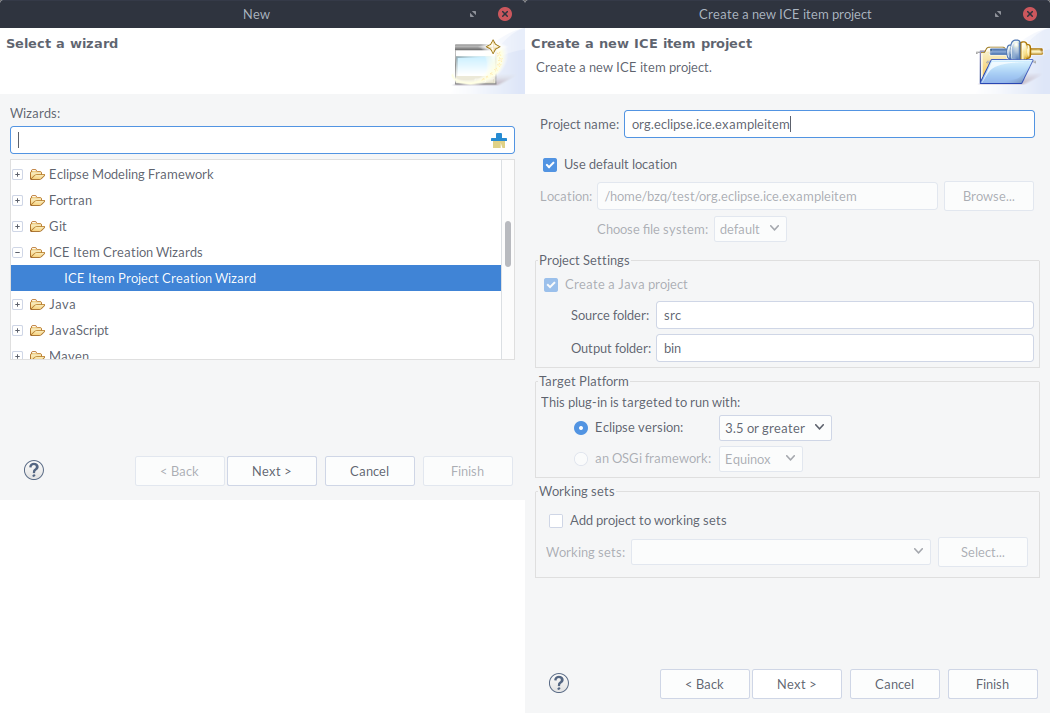
\includegraphics[width=\textwidth]{figures/comb12.png}
\label{fig:comb12}
\end{figure}

To create a new ICE Item project, navigate to \texttt{File $\rightarrow$ New
$\rightarrow$ Other}. Open the \texttt{ICE Item Creation Wizards} folder and 
select \texttt{ICE Item Creation Wizard}. You will be met with a standard new
project wizard page, in which you can name your project.  We will call ours
\texttt{org.eclipse.ice.fern}. Once you have named your project click the \texttt{Next>} button.
\begin{center} 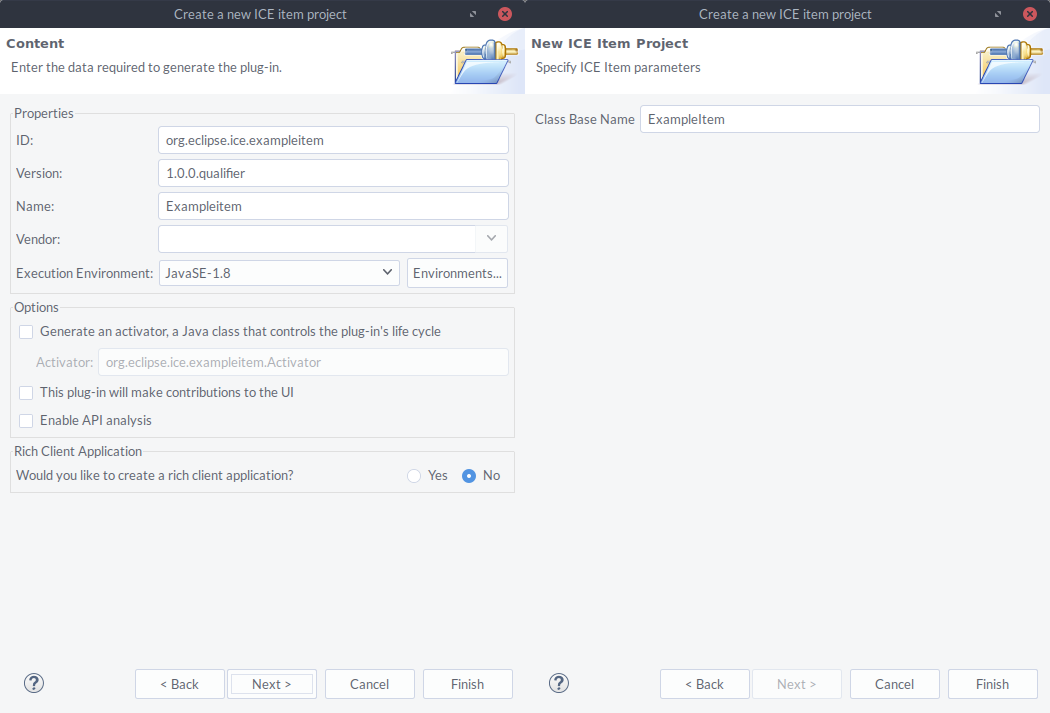
\includegraphics[width=\textwidth]{figures/comb23} \end{center}

The next dialog page enables you to customize the plugin-specific
portions of the project. For this tutorial, we will leave all the settings at
their defaults. Simply click \texttt{Next>} to move to the next page. 

On this page you need to tell the wizard what you want to use as a base
name for your item classes. We will call this one \texttt{Fern}. Then, we will
specify some information about how the item will handle input data.  FERN uses
the INI file format to specify data, so we will tell our item to use the built-in
functionality for INI files.  To do this select \texttt{INI} from the \texttt{File Format} dropdown.  

When you have entered all of the required information you can
click the \texttt{Finish} button to generate your new ICE Item plugin project.
When the project has finished generating you should be able to explore the code
that has been created.  Within the source directory there will be two packages,
each containing two Java classes:

\begin{itemize} 
    \item \texttt{org.eclipse.ice.fern.launcher} 
    \begin{itemize}
        \item \texttt{FernLauncher.java} 
        \item \texttt{FernLauncherBuilder.java}
    \end{itemize} 
    \item \texttt{org.eclipse.ice.fern.model} 
    \begin{itemize} 
        \item \texttt{FernModel.java} 
        \item \texttt{FernModelBuilder.java}
    \end{itemize} 
\end{itemize}

To add functionality to the project we need to edit
the \texttt{FernLauncher} and \texttt{FernModel} classes.

\subsection{Adding Functionality to the New Items}

\subsubsection{The Fern Model}

The \texttt{FernModel} will be responsible for creating and
validating input parameters for FERN, in the form of a new FERN input file.  In
order to make the generated code run there are several pieces of information that need to be changed.  First, we
will need to set up the basic Item idenfification information. This information
is set in the setupItemInfo() method. Modify the outputName to match the
following (or something of your choosing, with a .ini file extenstion).

\begin{lstlisting}[language=Java]
outputName = "fern_config.ini";
\end{lstlisting}

The String for the \emph{setName} method will serve as the display name
for this Item, so set it as \texttt{Fern Model}.
As for the String for \emph{setDescription}, this will also be used on the UI
for the Item, so provide some text like the following: \texttt{This Item constructs input files
for the FERN reaction network solver}. The export string will serve as the name
of the action that the user can select to write the provided data to file. Set
it to something like: \texttt{Export to INI}. You should now have a method that
looks like this:

\begin{lstlisting}[language=Java]
@Override
protected void setupItemInfo() {
	setName("Fern Model");
	setDescription("This Item constructs " +
	    "input files for the FERN reaction " +
	    "network solver"); 
	outputName = "fern_output.ini";   
	exportString = "Export to INI";
	allowedActions.add(0, exportString);
	ioFormat = "INI";
	defaultFileName = "";
}
\end{lstlisting}

The \emph{allowedActions.add()} line ensures that the export string is provided
to ICE as an allowed action, and displayed in the Item Process drop down.

With the identification information configured properly we can begin to
implement the Form for this FERN Model. This is done in the \emph{setupForm()}
method.
The generator has begun the process of implementing this method by instantiating
a Form for you to use, getting a reference to the IOService (which provides
IReader/IWriter realizations), and providing a commented out example of how to
fill out an ICE Form.

For this FERN input model, we want to add the following sections with data
entries: a network section with 
numSpecies, numReactions, numReactionGroups, massTol, fluxFrac, networkFile,
rateFile data entries, an initialConditions section with T9, startTime, endTime,
initialTimeStep, and density, and an output section with a single popFile
data entry.
To achieve this for this Item, we will need to add three
\texttt{DataComponents}, one for the network section, another for the
initialConditions section, and a final one for the outputs section. To each of
those DataComponents we will add appropriate IEntry instances for each of the data entries we have.

Add the following to your setupForm() method: 

\begin{lstlisting}[language=Java]

    // Create the network section
    DataComponent networkComp = new DataComponent();
    networkComp.setName("network");
    networkComp.setDescription("The parameters needed " +
        "to describe the nuclear " +
    	"reaction network"); 
    networkComp.setId(1);
    
    // Create the IEntries we need for this DataComponent
    StringEntry numSpecies = new StringEntry();
    numSpecies.setName("numSpecies");
    numSpecies.setDescription("The number of species to consider");
    numSpecies.setDefaultValue("16");
    
    StringEntry numReactions = new StringEntry();
    numReactions.setName("numReactions");
    numReactions.setDescription("The number of reactions to consider");
    numReactions.setDefaultValue("48");
    
    StringEntry numReactionGrps = new StringEntry();
    numReactionGrps.setName("numReactionsGroups");
    numReactionGrps.setDescription("The number of reaction " + 
    	"groups to consider"); 
    numReactionGrps.setDefaultValue("19");

    StringEntry massTol = new StringEntry();
    massTol.setName("massTol");
    massTol.setDescription("The mass tolerance to consider");
    massTol.setDefaultValue("1e-7");
    
    StringEntry fluxFrac = new StringEntry();
    fluxFrac.setName("fluxFrac");
    fluxFrac.setDescription("The flux fraction to consider");
    fluxFrac.setDefaultValue(".01");
    
    FileEntry networkFile = new FileEntry(".inp");
    networkFile.setProject(project);
    networkFile.setName("networkFile");
    networkFile.setDescription("The network file for this problem");
    
    FileEntry rateFile = new FileEntry(".data");
    rateFile.setProject(project);
    rateFile.setName("rateFile");
    rateFile.setDescription("The rate file for this problem");
    
    networkComp.addEntry(numSpecies);
    networkComp.addEntry(numReactions);
    networkComp.addEntry(numReactionGrps); 
    networkComp.addEntry(massTol);
    networkComp.addEntry(fluxFrac);
    networkComp.addEntry(networkFile);
    networkComp.addEntry(rateFile);
    
    // Create the initial conditions section
    DataComponent initConditionsComp = new DataComponent();
    initConditionsComp.setName("initialConditions");
    initConditionsComp.setId(2);
    initConditionsComp.setDescription("The parameters " +
    	"needed to describe the	initial " + 
    	"conditions for the problem");
    
    StringEntry t9 = new StringEntry();
    t9.setName("T9");
    t9.setDescription("The temperature in Kelvin x 10^9");
    t9.setDefaultValue("7.0");

    StringEntry startTime = new StringEntry();
    startTime.setName("startTime");
    startTime.setDescription("The start time for the simulation.");
    startTime.setDefaultValue("1e-20");

    StringEntry endTime = new StringEntry();
    endTime.setName("endTime");
    endTime.setDescription("The end time for the simulation");
    endTime.setDefaultValue("1e-3");

    StringEntry initialTimeStep = new StringEntry();
    initialTimeStep.setName("initialTimeStep");
    initialTimeStep.setDescription("The initial time step " + 
    	"for the simulation."); 
    initialTimeStep.setDefaultValue("1.2345e-22");

    StringEntry density = new StringEntry();
    density.setName("density");
    density.setDescription("The initial density.");
    density.setDefaultValue("1e8");
    
    initConditionsComp.addEntry(t9);
    initConditionsComp.addEntry(startTime);
    initConditionsComp.addEntry(endTime);
    initConditionsComp.addEntry(initialTimeStep);
    initConditionsComp.addEntry(density);
    
    // Create the outputs section
    DataComponent outputComp = new DataComponent();
    outputComp.setName("output");
    outputComp.setDescription("The parameters needed to output data.");
    outputComp.setId(3);
    
    StringEntry popFile = new StringEntry();
    popFile.setName("popFile");
    popFile.setDescription("The name of the output populations file");
    popFile.setDefaultValue("popFile.csv");
    
    outputComp.addEntry(popFile);
    
    // Add the components to the Form
    form.addComponent(networkComp);    
    form.addComponent(initConditionsComp);
    form.addComponent(outputComp);
    
\end{lstlisting}

Now we have a Form constructed for a typical FERN execution. 

The default generated implementation of the process method is sufficient to be
able to create new FERN INI input files. 

\subsubsection{Fern Launcher}
A FERN launcher handles the actual execution of the FERN application. The
generator creates the FernLauncher as a subclass of ICE's JobLauncher, which
provides a large array of features and functionality. As a subclass of
JobLauncher, the FernLauncher enables users to execute FERN locally or remotely.
To do so, we just need to add a small amount of
code that customizes the ICE job launching capabilities for FERN. 

The first bit of code to add to the FernLauncher specifies the name of the
actual Fern executable. In the setupItemInfo() method, set the execCommand to
the following: 
\begin{lstlisting}[language=Java]
execCommand = "${installDir}fern-exec";
\end{lstlisting}
This tells ICE that the FERN executable is called \texttt{fern-exec}, and to
set the overall execution command to it's install path plus the executable name.
The installDir flag will tell ICE to insert the user-specified executable
location (provided through the graphical form editor') into the execCommand,
with a trailing OS-specific path separator. This install directory is
specified through the Hosts Table on the editory. 

We also need to inform the JobLauncher what other files are involved in this
execution. To do that, the JobLauncher provides an addInputType() method. Add
the following to setupForm():
\begin{lstlisting}[language=Java]
addInputType("Network File", "networkFile", 
			"Network File Description", ".inp");
addInputType("Rate File", "rateFile", "
			Rate File Description", ".data");
\end{lstlisting}

And that should be it.
The generator has taken care of everything else for us.
We are now ready to launch ICE with our FERN plugin, and use the FERN Items we
have just created.


\chapter{Exploring Visualization in ICE}
\graphicspath{{../../geometryEditor/src/}}
\chapter{Paraview}

ICE features functionality for visualizing models using ParaView.

\section{Installation and Configuration}

ParaView use for ICE requires a Mac OS or Linux operating system, as ICE does
not currently support ParaView connections on Windows. You will also need an
installation of ParaView on your local machine. ParaView can be downloaded from
its \href{http://www.paraview.org/download/}{official website}. The ICE
development team recommends using the latest available version of ParaView,
currently 5.0 at the time of this writing. You will further need a custom
Python HTTP web server implementation, which can be downloaded from the
\href{http://eclipseice.ornl.gov/downloads/paraview/scripts/http_pvw_server.py}{Oak
Ridge website}.

\subsection{Configuring the ParaView Connection}

Once ParaView is running, ICE must be configured to connect to the server. This
is done through specifying a default connection in the ICE Preferences page.
This process only needs to be performed once. After initially creating the
connection, ICE will attempt to connect to ParaView on that port each time it is
launched.

To set the connection, select Window $\rightarrow$ Preferences\ldots in ICE's
menu bar. (On Mac OS X, Preferences\ldots is located under ICE instead of
Windows.) Select Visualization $\rightarrow$ ParaView in the tree on the left
side of the Preferences window.

\begin{center}
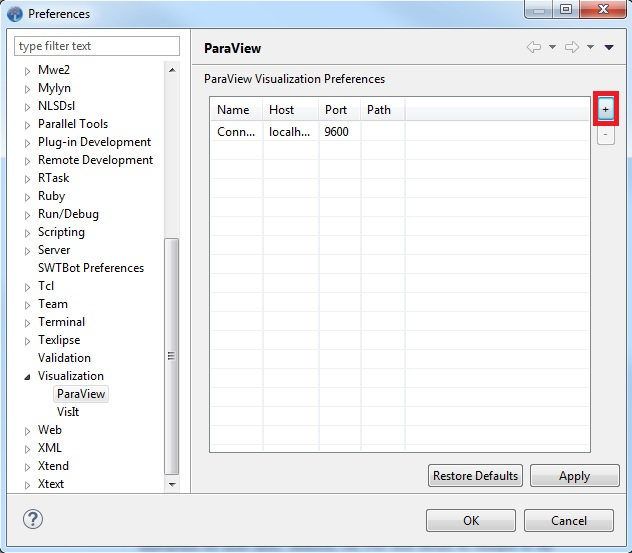
\includegraphics[width=12cm]{images/paraviewpreferencepage_ice}
\end{center}

Press the button with a ''+" symbol in the upper right (highlighted in the image
above) to add a new row to the table. Click on cells in the new row to edit
their values. 

\textbf{Name:} The connection's name. The default value will be fine.

\textbf{Host:} The hostname for the machine that will run ParaView. Use "localhost" if the machine running ICE will also be used to run ParaView.

\textbf{Port:} The port number on which the ParaView server will run. The default value will be fine, but if you change it, it must different from the Visualizer Port.

\textbf{Path:} The path to your ParaView installation. 

On Linux, the path will end with the top level folder into which ParaView was unzipped. For example, if you have a folder named ParaView on your desktop that contains the bin, doc, lib, and share folders, then your path would be /home/username/Desktop/ParaView. 

On Mac, the path will end with the folder containing your ParaView.app. For example, if you have installed ParaView to your Applications folder, the path will simply be /Applications

\textbf{Server Script Path:} The full path to the http_pvw_server.py file, ending with the folder containing it. For example if the file is on your desktop, the path might be /home/username/Desktop.

\textbf{Visualizer Port:} The port number for the ParaView web visualizer. The default value will be fine, but if you change it, then it must be different from the port number you provide for Port.

\textbf{Remote OS:} The operating system of the remote machine on which ParaView will be launched. If you want to launch ParaView on your local machine, ignore this cell. Otherwise, specify either "Linux" or "OSx".

\textbf{Remote ParaView Version Number:} The version of ParaView you are using. This may be ignored unless you are launching a remote ParaView session on a Linux machine. You can check your installation's version number by looking inside the top level \textbf{lib} folder. It will contain a folder named paraview- followed by the version number.

Once finished editing the cells in the new row, press Apply, then OK. ICE will
then launch the ParaView server and connect to it. If you are connecting to a remote machine, you will be prompted for permission to make the remote connection and asked for a password.

\section{Opening a ParaView File} 

To open a ParaView Plot Editor, a file that uses this editor must first be
placed in the Project Explorer. This view lists files imported into ICE. To
access the Project Explorer, use the the menu bar at the top of the window and
navigate to Window $\rightarrow$ Show View $\rightarrow$ Project Explorer.
Depending on the active Eclipse perspective, opening this view may require
selecting Other\ldots and finding the Project Explorer in the dialog under the
General category in the tree.

By default, the Project Explorer should automatically import the
ICEFiles/default and ICEFiles/itemDB folders. If it does not, or if you want to
import a different folder into ICE, right click in the Project Explorer and
select Import\ldots from the context menu. Then, select General $\rightarrow$
File System from the tree, and press the Next button. Select directories and/or
files to import into the Project Explorer, and enter which folder they should
be imported into, as shown below.

\begin{center}
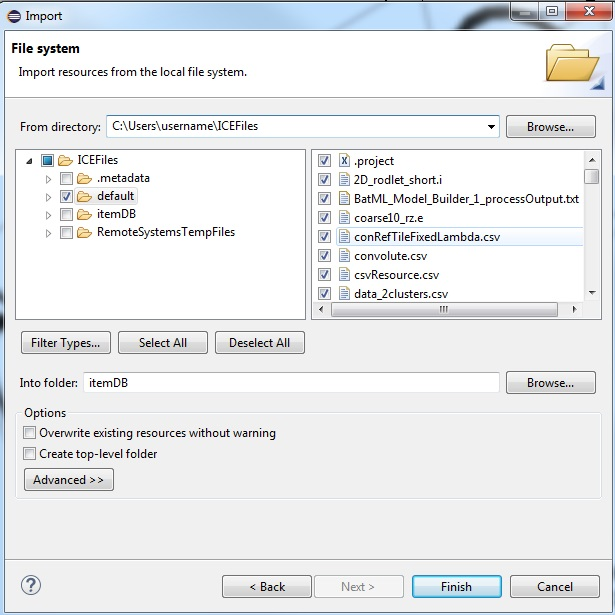
\includegraphics[width=12cm]{images/ImportFileDialog}
\end{center}

Once a file is in the Project Explorer, simply double click on it to open it in
ParaView. Local ParaView connections can only open local files, while remote ParaView connections can only open files on the remote host.

\subsection{Using ParaView}

\subsubsection{Camera Controls}

The Plot Editor allows the user to rotate the model by clicking and dragging
inside the display area or adjust the zoom by scrolling the mouse wheel.

\begin{center}
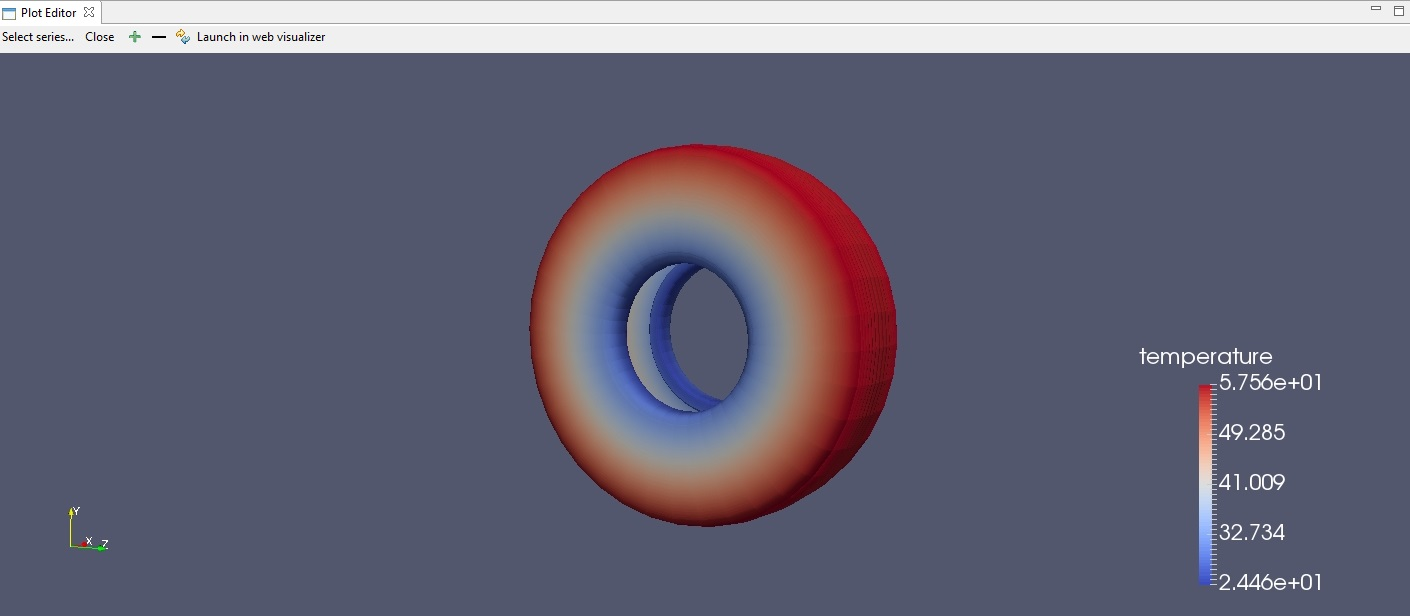
\includegraphics[width=12cm]{images/ParaViewPlotEditor}
\end{center}

The buttons in the upper left can also be used to manipulate the camera. The green plus sign will zoom in, while the black minus sign will zoom out. The green circular arrow button will reset the camera to its default position.

\subsubsection{Selecting the Plot}

Pressing the Select Series\ldots button will open a dialog which lists the
various plots in the opened file. Simply select one and click OK to open it. 

\begin{center}
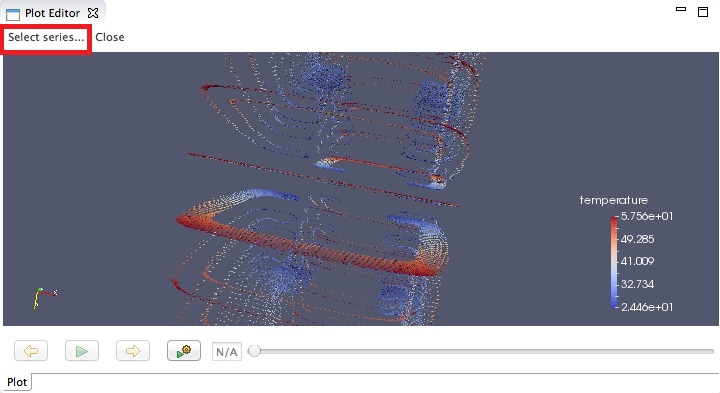
\includegraphics[width=12cm]{images/ParaViewPlotEditorSelectSeriesButton}
\end{center}

\subsubsection{Setting the Plot Representation} 

ParaView is capable of displaying plots in several different representations,
such as points or surfaces. To switch between plot type, right click inside the Plot
Editor's display area and select one of the listed options under the
Representation category in the context menu.

\begin{center}
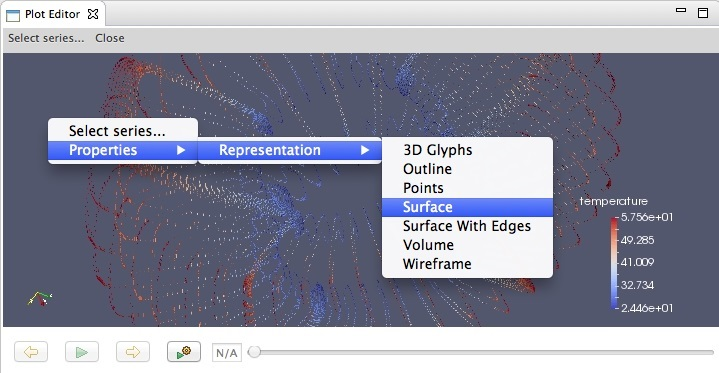
\includegraphics[width=12cm]{images/ParaViewRepresentationDropDown}
\end{center}

\subsubsection{Animation and Time Data}

The Plot Editor features a time slider widget at the bottom of the screen. 

\begin{center}
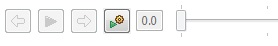
\includegraphics[width=12cm]{images/TimeSliderWidget}
\end{center}

The controls, in order of left to right, are:

1) Return to the previous time step.

2) Automatically play the plot as an animation by displaying the time steps
sequentially. 

3) Advance to the next time step. 

4) Opens an options menu that allows the user to set the playback speed, toggle
whether the animation should loop when it reaches the end, and set the plot to
the first or last time step.

5) A display for the current time step. It can be edited to set the plot to an
arbitrary time step. 

6) A slider that shows the current time step's position on the timeline. The
slider can be dragged around the timeline, setting the plot's time step
accordingly.

\section{Accessing a ParaView Web Server}

It is also possible to access the full ParaView web viewer application inside of
ICE. This allows for full access to all the web viewer's features.

\subsection{Accessing the Visualizer}

First, you must open a Plot Editor as described above.

\begin{center}
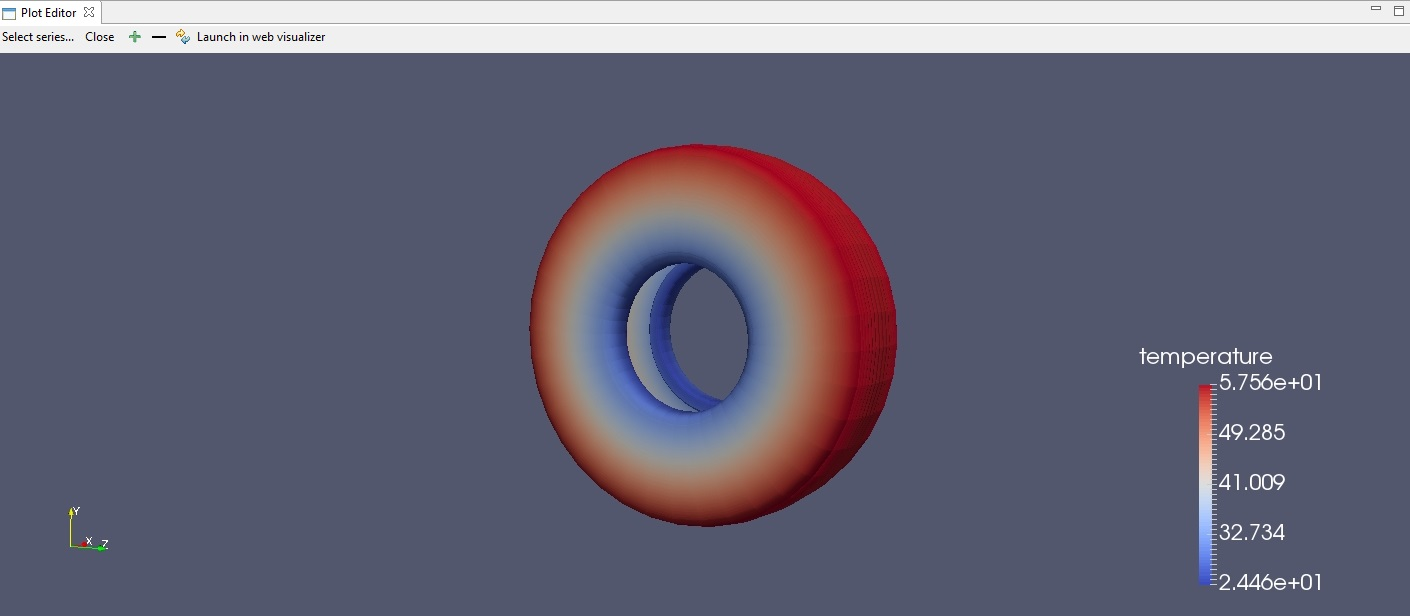
\includegraphics[width=12cm]{images/ParaViewPlotEditor}
\end{center}

Press the "Open in Web Visualizer" button in the top left to launch the web visualizer server and automatically open an internal web browser to view it.

\subsection{Using the Visualizer}

In order to load a data file, click the Show File List button as seen below.

\begin{center}
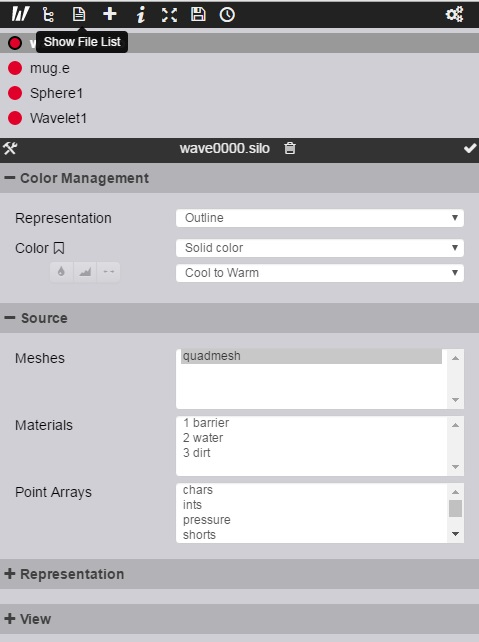
\includegraphics[width=12cm]{images/ParaViewVisualizer}
\end{center}

This will place the contents of the data directory into the side bar. For sessions, the data directory will be your ICE workspace. For a remote connection, this will be the folder containing the remote file you are visualizing. You may then double click on a file to load it into the model. 

You can click and drag the mouse to rotate the camera and right click followed
by dragging up or down to zoom. A full description of the visualizer's features
is beyond the scope of this tutorial, but see the official documentation
\href{http://www.paraview.org/ParaView3/Doc/Nightly/www/js-doc/index.html#!/guide/web_visualizer}{here}.

\graphicspath{{../../meshEditor/src/}}
\chapter{Paraview}

ICE features functionality for visualizing models using ParaView.

\section{Installation and Configuration}

ParaView use for ICE requires a Mac OS or Linux operating system, as ICE does
not currently support ParaView connections on Windows. You will also need an
installation of ParaView on your local machine. ParaView can be downloaded from
its \href{http://www.paraview.org/download/}{official website}. The ICE
development team recommends using the latest available version of ParaView,
currently 5.0 at the time of this writing. You will further need a custom
Python HTTP web server implementation, which can be downloaded from the
\href{http://eclipseice.ornl.gov/downloads/paraview/scripts/http_pvw_server.py}{Oak
Ridge website}.

\subsection{Configuring the ParaView Connection}

Once ParaView is running, ICE must be configured to connect to the server. This
is done through specifying a default connection in the ICE Preferences page.
This process only needs to be performed once. After initially creating the
connection, ICE will attempt to connect to ParaView on that port each time it is
launched.

To set the connection, select Window $\rightarrow$ Preferences\ldots in ICE's
menu bar. (On Mac OS X, Preferences\ldots is located under ICE instead of
Windows.) Select Visualization $\rightarrow$ ParaView in the tree on the left
side of the Preferences window.

\begin{center}
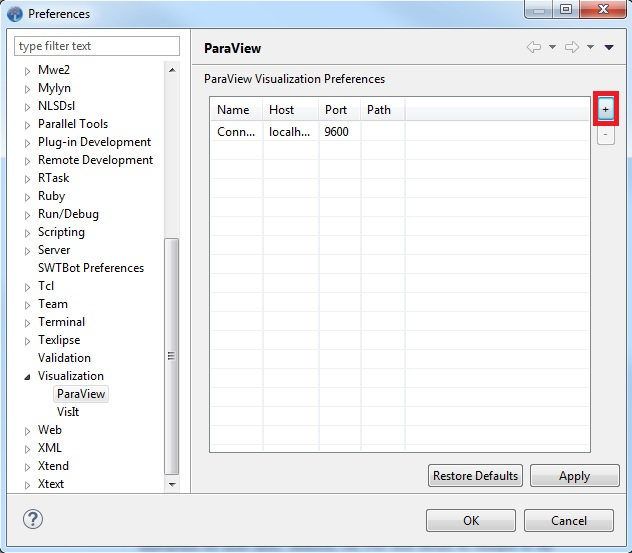
\includegraphics[width=12cm]{images/paraviewpreferencepage_ice}
\end{center}

Press the button with a ''+" symbol in the upper right (highlighted in the image
above) to add a new row to the table. Click on cells in the new row to edit
their values. 

\textbf{Name:} The connection's name. The default value will be fine.

\textbf{Host:} The hostname for the machine that will run ParaView. Use "localhost" if the machine running ICE will also be used to run ParaView.

\textbf{Port:} The port number on which the ParaView server will run. The default value will be fine, but if you change it, it must different from the Visualizer Port.

\textbf{Path:} The path to your ParaView installation. 

On Linux, the path will end with the top level folder into which ParaView was unzipped. For example, if you have a folder named ParaView on your desktop that contains the bin, doc, lib, and share folders, then your path would be /home/username/Desktop/ParaView. 

On Mac, the path will end with the folder containing your ParaView.app. For example, if you have installed ParaView to your Applications folder, the path will simply be /Applications

\textbf{Server Script Path:} The full path to the http_pvw_server.py file, ending with the folder containing it. For example if the file is on your desktop, the path might be /home/username/Desktop.

\textbf{Visualizer Port:} The port number for the ParaView web visualizer. The default value will be fine, but if you change it, then it must be different from the port number you provide for Port.

\textbf{Remote OS:} The operating system of the remote machine on which ParaView will be launched. If you want to launch ParaView on your local machine, ignore this cell. Otherwise, specify either "Linux" or "OSx".

\textbf{Remote ParaView Version Number:} The version of ParaView you are using. This may be ignored unless you are launching a remote ParaView session on a Linux machine. You can check your installation's version number by looking inside the top level \textbf{lib} folder. It will contain a folder named paraview- followed by the version number.

Once finished editing the cells in the new row, press Apply, then OK. ICE will
then launch the ParaView server and connect to it. If you are connecting to a remote machine, you will be prompted for permission to make the remote connection and asked for a password.

\section{Opening a ParaView File} 

To open a ParaView Plot Editor, a file that uses this editor must first be
placed in the Project Explorer. This view lists files imported into ICE. To
access the Project Explorer, use the the menu bar at the top of the window and
navigate to Window $\rightarrow$ Show View $\rightarrow$ Project Explorer.
Depending on the active Eclipse perspective, opening this view may require
selecting Other\ldots and finding the Project Explorer in the dialog under the
General category in the tree.

By default, the Project Explorer should automatically import the
ICEFiles/default and ICEFiles/itemDB folders. If it does not, or if you want to
import a different folder into ICE, right click in the Project Explorer and
select Import\ldots from the context menu. Then, select General $\rightarrow$
File System from the tree, and press the Next button. Select directories and/or
files to import into the Project Explorer, and enter which folder they should
be imported into, as shown below.

\begin{center}
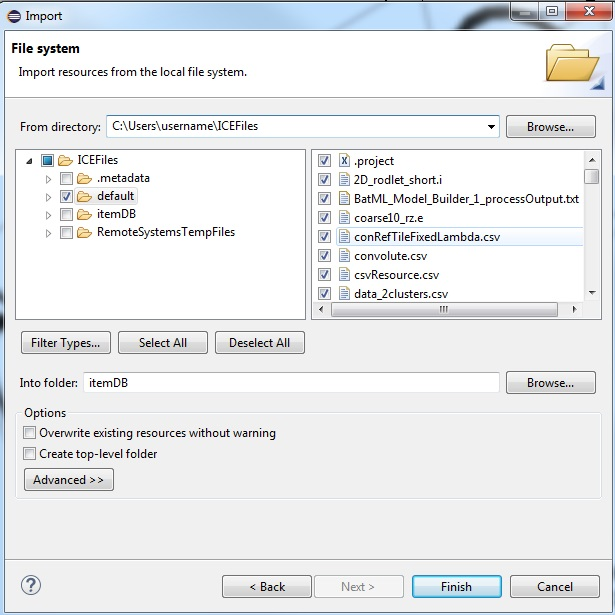
\includegraphics[width=12cm]{images/ImportFileDialog}
\end{center}

Once a file is in the Project Explorer, simply double click on it to open it in
ParaView. Local ParaView connections can only open local files, while remote ParaView connections can only open files on the remote host.

\subsection{Using ParaView}

\subsubsection{Camera Controls}

The Plot Editor allows the user to rotate the model by clicking and dragging
inside the display area or adjust the zoom by scrolling the mouse wheel.

\begin{center}
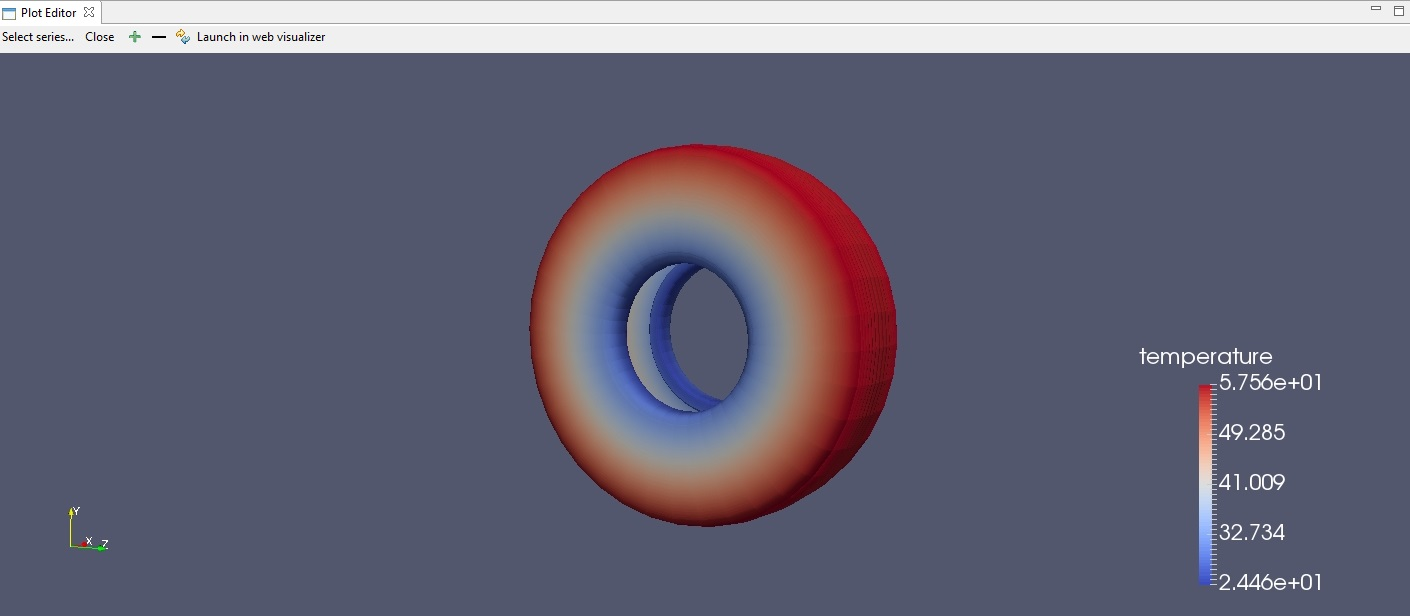
\includegraphics[width=12cm]{images/ParaViewPlotEditor}
\end{center}

The buttons in the upper left can also be used to manipulate the camera. The green plus sign will zoom in, while the black minus sign will zoom out. The green circular arrow button will reset the camera to its default position.

\subsubsection{Selecting the Plot}

Pressing the Select Series\ldots button will open a dialog which lists the
various plots in the opened file. Simply select one and click OK to open it. 

\begin{center}
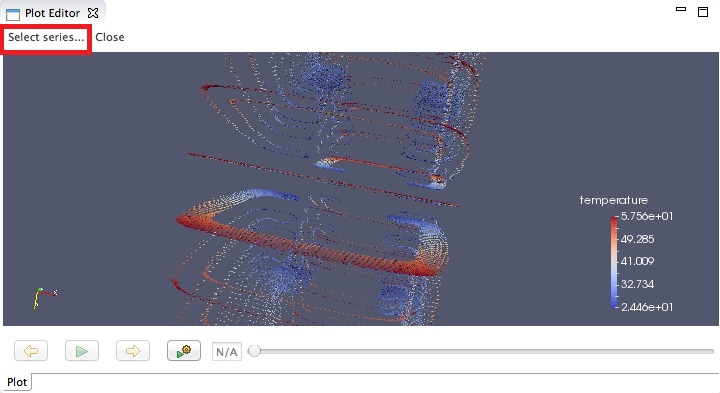
\includegraphics[width=12cm]{images/ParaViewPlotEditorSelectSeriesButton}
\end{center}

\subsubsection{Setting the Plot Representation} 

ParaView is capable of displaying plots in several different representations,
such as points or surfaces. To switch between plot type, right click inside the Plot
Editor's display area and select one of the listed options under the
Representation category in the context menu.

\begin{center}
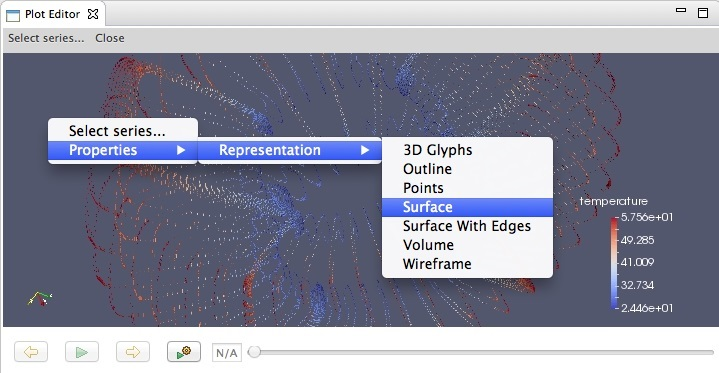
\includegraphics[width=12cm]{images/ParaViewRepresentationDropDown}
\end{center}

\subsubsection{Animation and Time Data}

The Plot Editor features a time slider widget at the bottom of the screen. 

\begin{center}
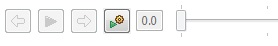
\includegraphics[width=12cm]{images/TimeSliderWidget}
\end{center}

The controls, in order of left to right, are:

1) Return to the previous time step.

2) Automatically play the plot as an animation by displaying the time steps
sequentially. 

3) Advance to the next time step. 

4) Opens an options menu that allows the user to set the playback speed, toggle
whether the animation should loop when it reaches the end, and set the plot to
the first or last time step.

5) A display for the current time step. It can be edited to set the plot to an
arbitrary time step. 

6) A slider that shows the current time step's position on the timeline. The
slider can be dragged around the timeline, setting the plot's time step
accordingly.

\section{Accessing a ParaView Web Server}

It is also possible to access the full ParaView web viewer application inside of
ICE. This allows for full access to all the web viewer's features.

\subsection{Accessing the Visualizer}

First, you must open a Plot Editor as described above.

\begin{center}
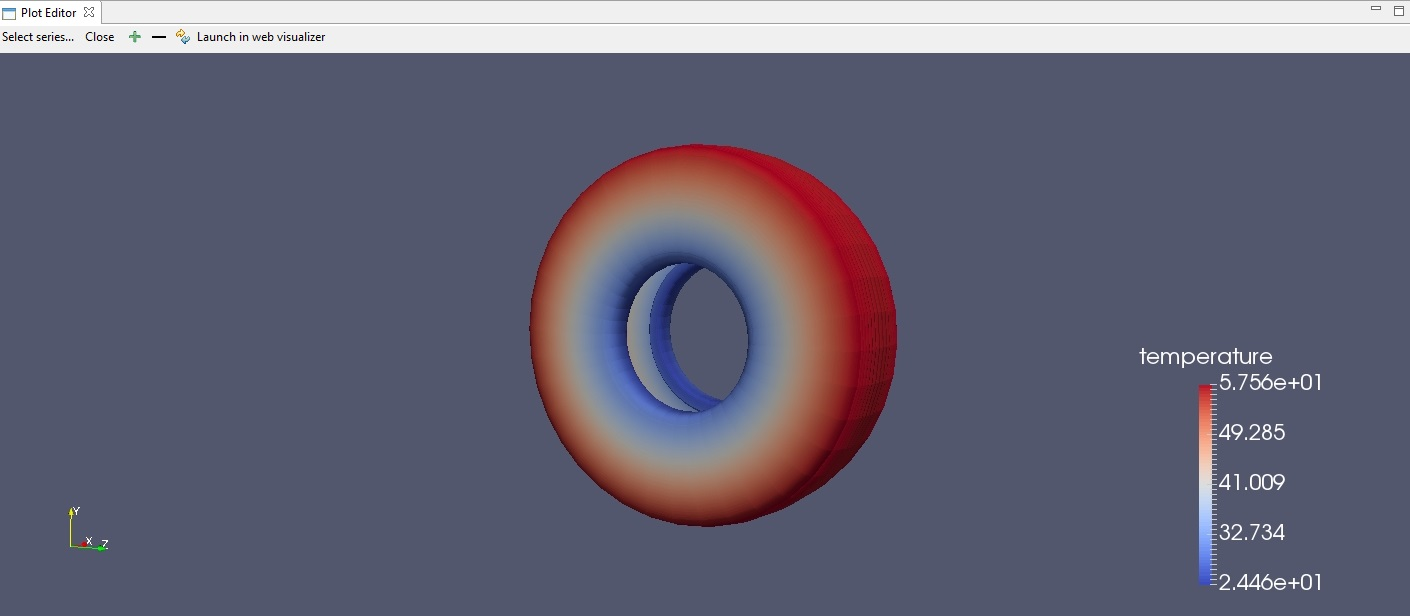
\includegraphics[width=12cm]{images/ParaViewPlotEditor}
\end{center}

Press the "Open in Web Visualizer" button in the top left to launch the web visualizer server and automatically open an internal web browser to view it.

\subsection{Using the Visualizer}

In order to load a data file, click the Show File List button as seen below.

\begin{center}
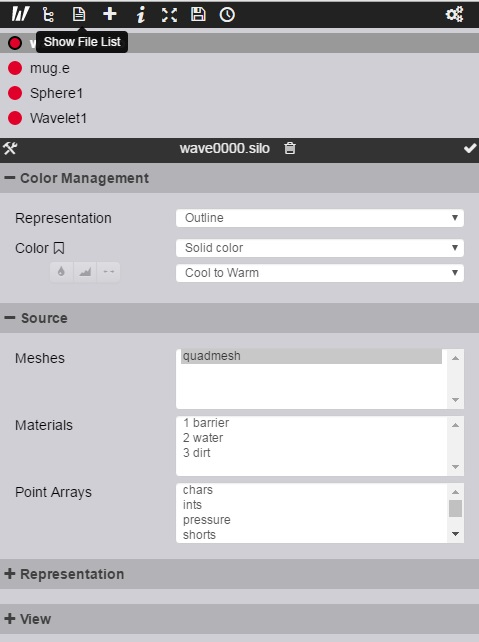
\includegraphics[width=12cm]{images/ParaViewVisualizer}
\end{center}

This will place the contents of the data directory into the side bar. For sessions, the data directory will be your ICE workspace. For a remote connection, this will be the folder containing the remote file you are visualizing. You may then double click on a file to load it into the model. 

You can click and drag the mouse to rotate the camera and right click followed
by dragging up or down to zoom. A full description of the visualizer's features
is beyond the scope of this tutorial, but see the official documentation
\href{http://www.paraview.org/ParaView3/Doc/Nightly/www/js-doc/index.html#!/guide/web_visualizer}{here}.

\graphicspath{{../../visualization/src/}}
\section{Creating an ICE Item} 

This tutorial will teach you how to
create your own ICE Items via the built-in tools within ICE.  To demonstrate
these tools, we will walk through the development of a dashboard for the
FERN code, a fast, efficient nuclear reaction network solver. 

After creating a new ICE Item plugin project, we will demonstrate how to
provide a few lines of code to create an editor for
input files for FERN. After that we will show how a small amount of code can be
used to create a job launcher that is customized to execute FERN locally. We
will also show how to launch FERN remotely.

\subsection{Creating the Project}

\begin{figure}[h]
\centering
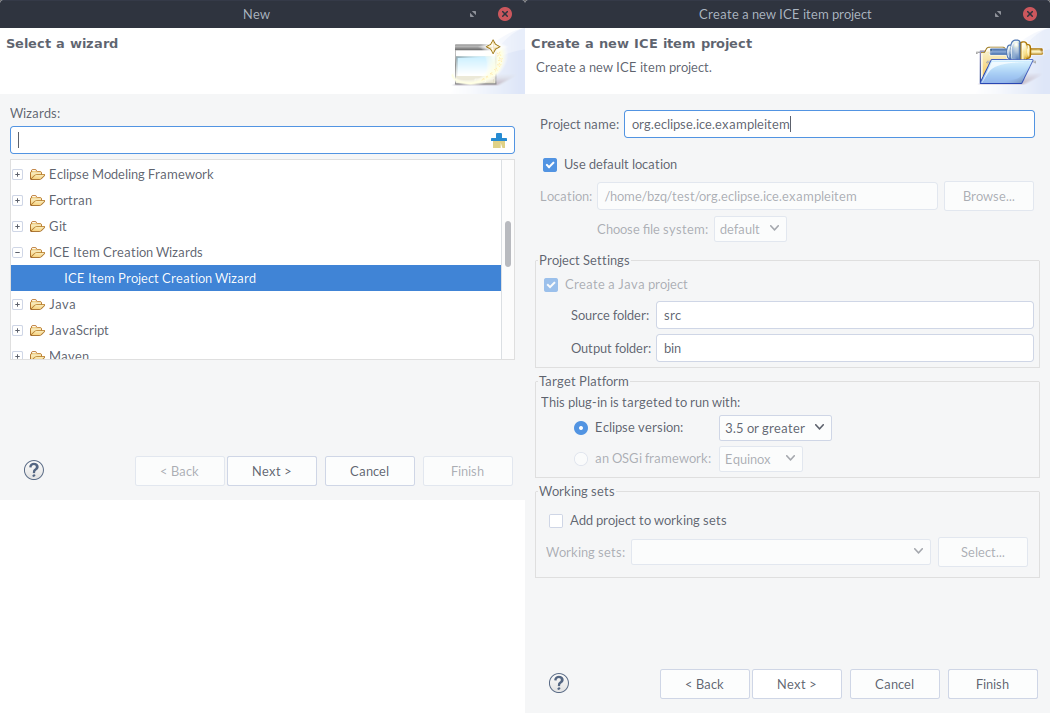
\includegraphics[width=\textwidth]{figures/comb12.png}
\label{fig:comb12}
\end{figure}

To create a new ICE Item project, navigate to \texttt{File $\rightarrow$ New
$\rightarrow$ Other}. Open the \texttt{ICE Item Creation Wizards} folder and 
select \texttt{ICE Item Creation Wizard}. You will be met with a standard new
project wizard page, in which you can name your project.  We will call ours
\texttt{org.eclipse.ice.fern}. Once you have named your project click the \texttt{Next>} button.
\begin{center} 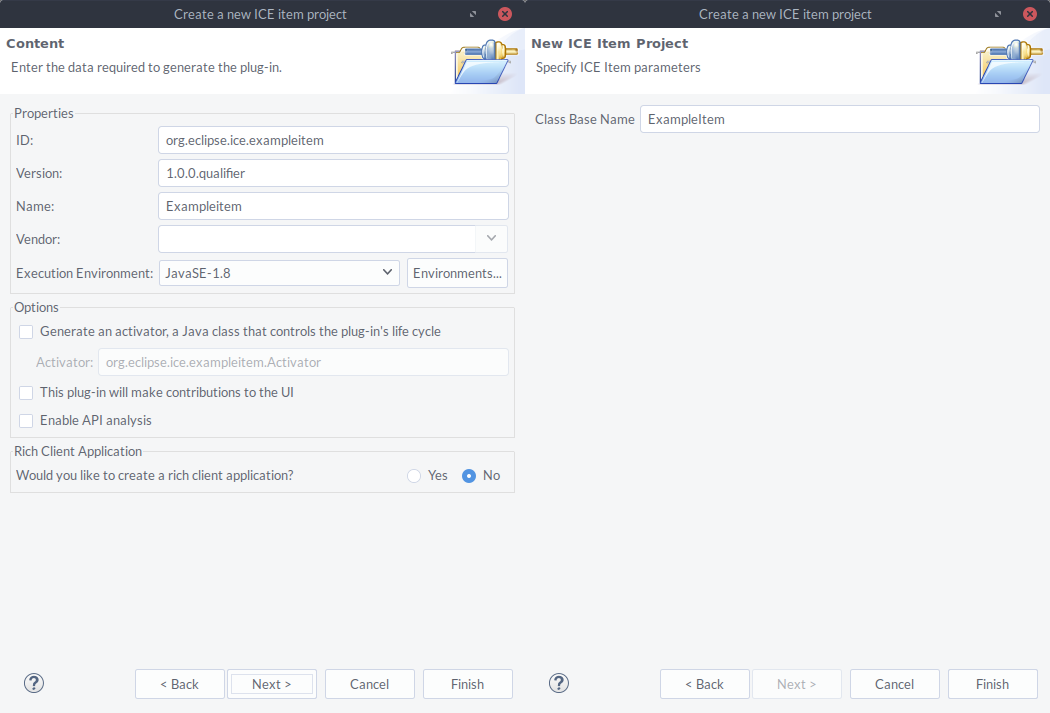
\includegraphics[width=\textwidth]{figures/comb23} \end{center}

The next dialog page enables you to customize the plugin-specific
portions of the project. For this tutorial, we will leave all the settings at
their defaults. Simply click \texttt{Next>} to move to the next page. 

On this page you need to tell the wizard what you want to use as a base
name for your item classes. We will call this one \texttt{Fern}. Then, we will
specify some information about how the item will handle input data.  FERN uses
the INI file format to specify data, so we will tell our item to use the built-in
functionality for INI files.  To do this select \texttt{INI} from the \texttt{File Format} dropdown.  

When you have entered all of the required information you can
click the \texttt{Finish} button to generate your new ICE Item plugin project.
When the project has finished generating you should be able to explore the code
that has been created.  Within the source directory there will be two packages,
each containing two Java classes:

\begin{itemize} 
    \item \texttt{org.eclipse.ice.fern.launcher} 
    \begin{itemize}
        \item \texttt{FernLauncher.java} 
        \item \texttt{FernLauncherBuilder.java}
    \end{itemize} 
    \item \texttt{org.eclipse.ice.fern.model} 
    \begin{itemize} 
        \item \texttt{FernModel.java} 
        \item \texttt{FernModelBuilder.java}
    \end{itemize} 
\end{itemize}

To add functionality to the project we need to edit
the \texttt{FernLauncher} and \texttt{FernModel} classes.

\subsection{Adding Functionality to the New Items}

\subsubsection{The Fern Model}

The \texttt{FernModel} will be responsible for creating and
validating input parameters for FERN, in the form of a new FERN input file.  In
order to make the generated code run there are several pieces of information that need to be changed.  First, we
will need to set up the basic Item idenfification information. This information
is set in the setupItemInfo() method. Modify the outputName to match the
following (or something of your choosing, with a .ini file extenstion).

\begin{lstlisting}[language=Java]
outputName = "fern_config.ini";
\end{lstlisting}

The String for the \emph{setName} method will serve as the display name
for this Item, so set it as \texttt{Fern Model}.
As for the String for \emph{setDescription}, this will also be used on the UI
for the Item, so provide some text like the following: \texttt{This Item constructs input files
for the FERN reaction network solver}. The export string will serve as the name
of the action that the user can select to write the provided data to file. Set
it to something like: \texttt{Export to INI}. You should now have a method that
looks like this:

\begin{lstlisting}[language=Java]
@Override
protected void setupItemInfo() {
	setName("Fern Model");
	setDescription("This Item constructs " +
	    "input files for the FERN reaction " +
	    "network solver"); 
	outputName = "fern_output.ini";   
	exportString = "Export to INI";
	allowedActions.add(0, exportString);
	ioFormat = "INI";
	defaultFileName = "";
}
\end{lstlisting}

The \emph{allowedActions.add()} line ensures that the export string is provided
to ICE as an allowed action, and displayed in the Item Process drop down.

With the identification information configured properly we can begin to
implement the Form for this FERN Model. This is done in the \emph{setupForm()}
method.
The generator has begun the process of implementing this method by instantiating
a Form for you to use, getting a reference to the IOService (which provides
IReader/IWriter realizations), and providing a commented out example of how to
fill out an ICE Form.

For this FERN input model, we want to add the following sections with data
entries: a network section with 
numSpecies, numReactions, numReactionGroups, massTol, fluxFrac, networkFile,
rateFile data entries, an initialConditions section with T9, startTime, endTime,
initialTimeStep, and density, and an output section with a single popFile
data entry.
To achieve this for this Item, we will need to add three
\texttt{DataComponents}, one for the network section, another for the
initialConditions section, and a final one for the outputs section. To each of
those DataComponents we will add appropriate IEntry instances for each of the data entries we have.

Add the following to your setupForm() method: 

\begin{lstlisting}[language=Java]

    // Create the network section
    DataComponent networkComp = new DataComponent();
    networkComp.setName("network");
    networkComp.setDescription("The parameters needed " +
        "to describe the nuclear " +
    	"reaction network"); 
    networkComp.setId(1);
    
    // Create the IEntries we need for this DataComponent
    StringEntry numSpecies = new StringEntry();
    numSpecies.setName("numSpecies");
    numSpecies.setDescription("The number of species to consider");
    numSpecies.setDefaultValue("16");
    
    StringEntry numReactions = new StringEntry();
    numReactions.setName("numReactions");
    numReactions.setDescription("The number of reactions to consider");
    numReactions.setDefaultValue("48");
    
    StringEntry numReactionGrps = new StringEntry();
    numReactionGrps.setName("numReactionsGroups");
    numReactionGrps.setDescription("The number of reaction " + 
    	"groups to consider"); 
    numReactionGrps.setDefaultValue("19");

    StringEntry massTol = new StringEntry();
    massTol.setName("massTol");
    massTol.setDescription("The mass tolerance to consider");
    massTol.setDefaultValue("1e-7");
    
    StringEntry fluxFrac = new StringEntry();
    fluxFrac.setName("fluxFrac");
    fluxFrac.setDescription("The flux fraction to consider");
    fluxFrac.setDefaultValue(".01");
    
    FileEntry networkFile = new FileEntry(".inp");
    networkFile.setProject(project);
    networkFile.setName("networkFile");
    networkFile.setDescription("The network file for this problem");
    
    FileEntry rateFile = new FileEntry(".data");
    rateFile.setProject(project);
    rateFile.setName("rateFile");
    rateFile.setDescription("The rate file for this problem");
    
    networkComp.addEntry(numSpecies);
    networkComp.addEntry(numReactions);
    networkComp.addEntry(numReactionGrps); 
    networkComp.addEntry(massTol);
    networkComp.addEntry(fluxFrac);
    networkComp.addEntry(networkFile);
    networkComp.addEntry(rateFile);
    
    // Create the initial conditions section
    DataComponent initConditionsComp = new DataComponent();
    initConditionsComp.setName("initialConditions");
    initConditionsComp.setId(2);
    initConditionsComp.setDescription("The parameters " +
    	"needed to describe the	initial " + 
    	"conditions for the problem");
    
    StringEntry t9 = new StringEntry();
    t9.setName("T9");
    t9.setDescription("The temperature in Kelvin x 10^9");
    t9.setDefaultValue("7.0");

    StringEntry startTime = new StringEntry();
    startTime.setName("startTime");
    startTime.setDescription("The start time for the simulation.");
    startTime.setDefaultValue("1e-20");

    StringEntry endTime = new StringEntry();
    endTime.setName("endTime");
    endTime.setDescription("The end time for the simulation");
    endTime.setDefaultValue("1e-3");

    StringEntry initialTimeStep = new StringEntry();
    initialTimeStep.setName("initialTimeStep");
    initialTimeStep.setDescription("The initial time step " + 
    	"for the simulation."); 
    initialTimeStep.setDefaultValue("1.2345e-22");

    StringEntry density = new StringEntry();
    density.setName("density");
    density.setDescription("The initial density.");
    density.setDefaultValue("1e8");
    
    initConditionsComp.addEntry(t9);
    initConditionsComp.addEntry(startTime);
    initConditionsComp.addEntry(endTime);
    initConditionsComp.addEntry(initialTimeStep);
    initConditionsComp.addEntry(density);
    
    // Create the outputs section
    DataComponent outputComp = new DataComponent();
    outputComp.setName("output");
    outputComp.setDescription("The parameters needed to output data.");
    outputComp.setId(3);
    
    StringEntry popFile = new StringEntry();
    popFile.setName("popFile");
    popFile.setDescription("The name of the output populations file");
    popFile.setDefaultValue("popFile.csv");
    
    outputComp.addEntry(popFile);
    
    // Add the components to the Form
    form.addComponent(networkComp);    
    form.addComponent(initConditionsComp);
    form.addComponent(outputComp);
    
\end{lstlisting}

Now we have a Form constructed for a typical FERN execution. 

The default generated implementation of the process method is sufficient to be
able to create new FERN INI input files. 

\subsubsection{Fern Launcher}
A FERN launcher handles the actual execution of the FERN application. The
generator creates the FernLauncher as a subclass of ICE's JobLauncher, which
provides a large array of features and functionality. As a subclass of
JobLauncher, the FernLauncher enables users to execute FERN locally or remotely.
To do so, we just need to add a small amount of
code that customizes the ICE job launching capabilities for FERN. 

The first bit of code to add to the FernLauncher specifies the name of the
actual Fern executable. In the setupItemInfo() method, set the execCommand to
the following: 
\begin{lstlisting}[language=Java]
execCommand = "${installDir}fern-exec";
\end{lstlisting}
This tells ICE that the FERN executable is called \texttt{fern-exec}, and to
set the overall execution command to it's install path plus the executable name.
The installDir flag will tell ICE to insert the user-specified executable
location (provided through the graphical form editor') into the execCommand,
with a trailing OS-specific path separator. This install directory is
specified through the Hosts Table on the editory. 

We also need to inform the JobLauncher what other files are involved in this
execution. To do that, the JobLauncher provides an addInputType() method. Add
the following to setupForm():
\begin{lstlisting}[language=Java]
addInputType("Network File", "networkFile", 
			"Network File Description", ".inp");
addInputType("Rate File", "rateFile", "
			Rate File Description", ".data");
\end{lstlisting}

And that should be it.
The generator has taken care of everything else for us.
We are now ready to launch ICE with our FERN plugin, and use the FERN Items we
have just created.


\chapter{Extending ICE}
\graphicspath{{../../scripting/src/}}
\lstset{inputpath=../../scripting/src/}
\chapter{Paraview}

ICE features functionality for visualizing models using ParaView.

\section{Installation and Configuration}

ParaView use for ICE requires a Mac OS or Linux operating system, as ICE does
not currently support ParaView connections on Windows. You will also need an
installation of ParaView on your local machine. ParaView can be downloaded from
its \href{http://www.paraview.org/download/}{official website}. The ICE
development team recommends using the latest available version of ParaView,
currently 5.0 at the time of this writing. You will further need a custom
Python HTTP web server implementation, which can be downloaded from the
\href{http://eclipseice.ornl.gov/downloads/paraview/scripts/http_pvw_server.py}{Oak
Ridge website}.

\subsection{Configuring the ParaView Connection}

Once ParaView is running, ICE must be configured to connect to the server. This
is done through specifying a default connection in the ICE Preferences page.
This process only needs to be performed once. After initially creating the
connection, ICE will attempt to connect to ParaView on that port each time it is
launched.

To set the connection, select Window $\rightarrow$ Preferences\ldots in ICE's
menu bar. (On Mac OS X, Preferences\ldots is located under ICE instead of
Windows.) Select Visualization $\rightarrow$ ParaView in the tree on the left
side of the Preferences window.

\begin{center}
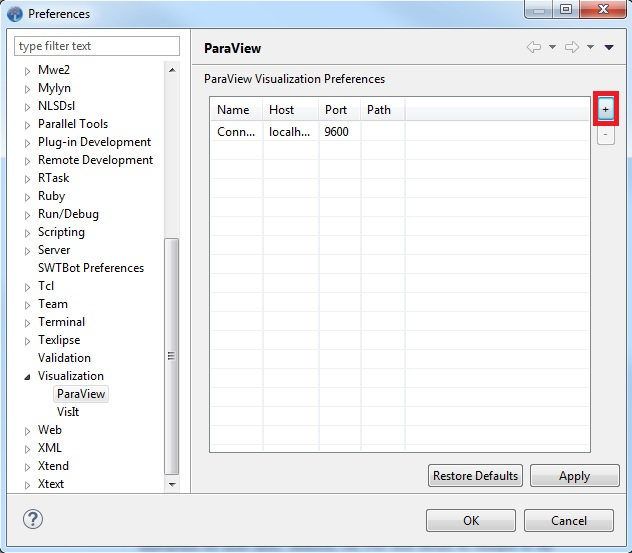
\includegraphics[width=12cm]{images/paraviewpreferencepage_ice}
\end{center}

Press the button with a ''+" symbol in the upper right (highlighted in the image
above) to add a new row to the table. Click on cells in the new row to edit
their values. 

\textbf{Name:} The connection's name. The default value will be fine.

\textbf{Host:} The hostname for the machine that will run ParaView. Use "localhost" if the machine running ICE will also be used to run ParaView.

\textbf{Port:} The port number on which the ParaView server will run. The default value will be fine, but if you change it, it must different from the Visualizer Port.

\textbf{Path:} The path to your ParaView installation. 

On Linux, the path will end with the top level folder into which ParaView was unzipped. For example, if you have a folder named ParaView on your desktop that contains the bin, doc, lib, and share folders, then your path would be /home/username/Desktop/ParaView. 

On Mac, the path will end with the folder containing your ParaView.app. For example, if you have installed ParaView to your Applications folder, the path will simply be /Applications

\textbf{Server Script Path:} The full path to the http_pvw_server.py file, ending with the folder containing it. For example if the file is on your desktop, the path might be /home/username/Desktop.

\textbf{Visualizer Port:} The port number for the ParaView web visualizer. The default value will be fine, but if you change it, then it must be different from the port number you provide for Port.

\textbf{Remote OS:} The operating system of the remote machine on which ParaView will be launched. If you want to launch ParaView on your local machine, ignore this cell. Otherwise, specify either "Linux" or "OSx".

\textbf{Remote ParaView Version Number:} The version of ParaView you are using. This may be ignored unless you are launching a remote ParaView session on a Linux machine. You can check your installation's version number by looking inside the top level \textbf{lib} folder. It will contain a folder named paraview- followed by the version number.

Once finished editing the cells in the new row, press Apply, then OK. ICE will
then launch the ParaView server and connect to it. If you are connecting to a remote machine, you will be prompted for permission to make the remote connection and asked for a password.

\section{Opening a ParaView File} 

To open a ParaView Plot Editor, a file that uses this editor must first be
placed in the Project Explorer. This view lists files imported into ICE. To
access the Project Explorer, use the the menu bar at the top of the window and
navigate to Window $\rightarrow$ Show View $\rightarrow$ Project Explorer.
Depending on the active Eclipse perspective, opening this view may require
selecting Other\ldots and finding the Project Explorer in the dialog under the
General category in the tree.

By default, the Project Explorer should automatically import the
ICEFiles/default and ICEFiles/itemDB folders. If it does not, or if you want to
import a different folder into ICE, right click in the Project Explorer and
select Import\ldots from the context menu. Then, select General $\rightarrow$
File System from the tree, and press the Next button. Select directories and/or
files to import into the Project Explorer, and enter which folder they should
be imported into, as shown below.

\begin{center}
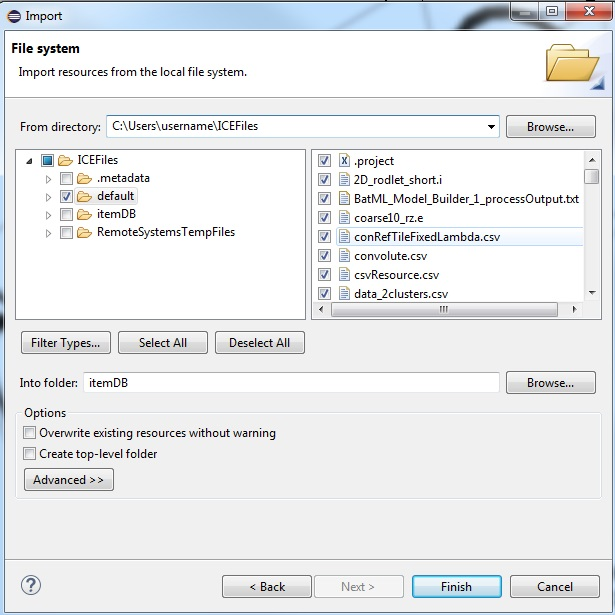
\includegraphics[width=12cm]{images/ImportFileDialog}
\end{center}

Once a file is in the Project Explorer, simply double click on it to open it in
ParaView. Local ParaView connections can only open local files, while remote ParaView connections can only open files on the remote host.

\subsection{Using ParaView}

\subsubsection{Camera Controls}

The Plot Editor allows the user to rotate the model by clicking and dragging
inside the display area or adjust the zoom by scrolling the mouse wheel.

\begin{center}
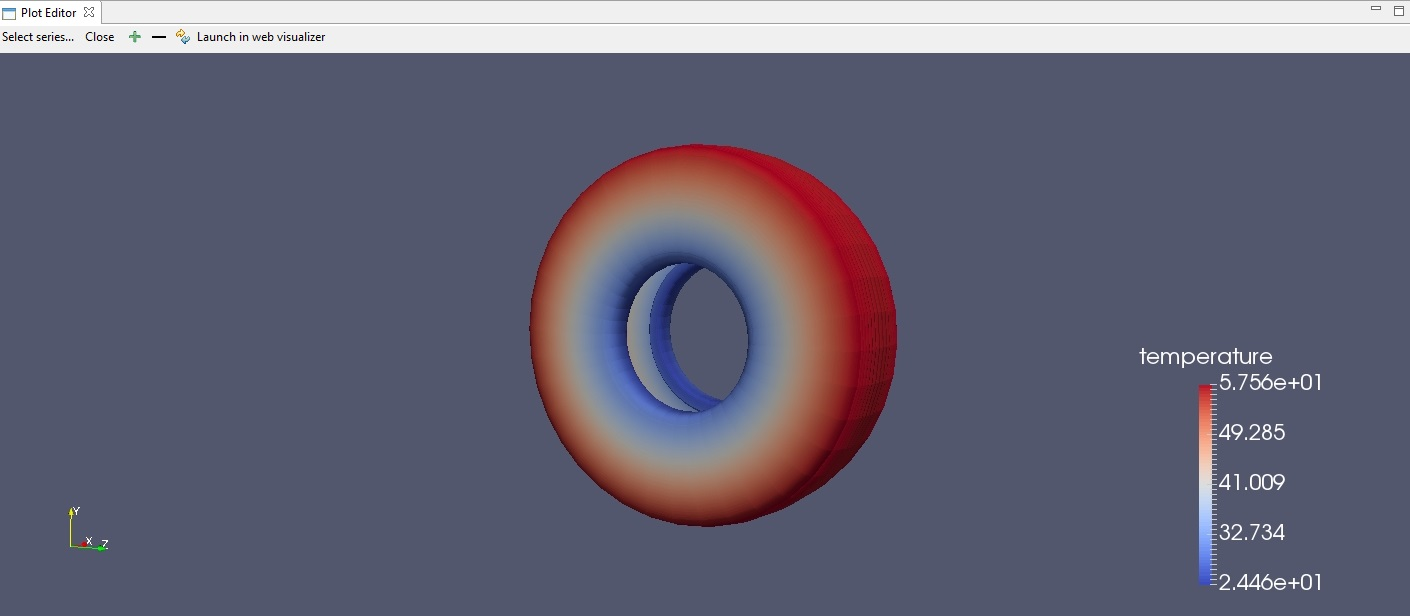
\includegraphics[width=12cm]{images/ParaViewPlotEditor}
\end{center}

The buttons in the upper left can also be used to manipulate the camera. The green plus sign will zoom in, while the black minus sign will zoom out. The green circular arrow button will reset the camera to its default position.

\subsubsection{Selecting the Plot}

Pressing the Select Series\ldots button will open a dialog which lists the
various plots in the opened file. Simply select one and click OK to open it. 

\begin{center}
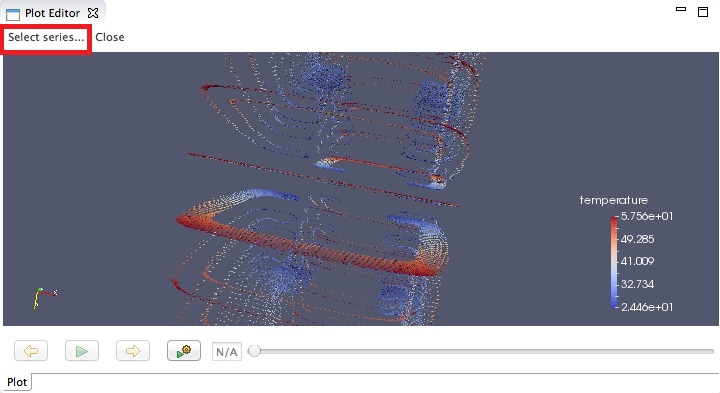
\includegraphics[width=12cm]{images/ParaViewPlotEditorSelectSeriesButton}
\end{center}

\subsubsection{Setting the Plot Representation} 

ParaView is capable of displaying plots in several different representations,
such as points or surfaces. To switch between plot type, right click inside the Plot
Editor's display area and select one of the listed options under the
Representation category in the context menu.

\begin{center}
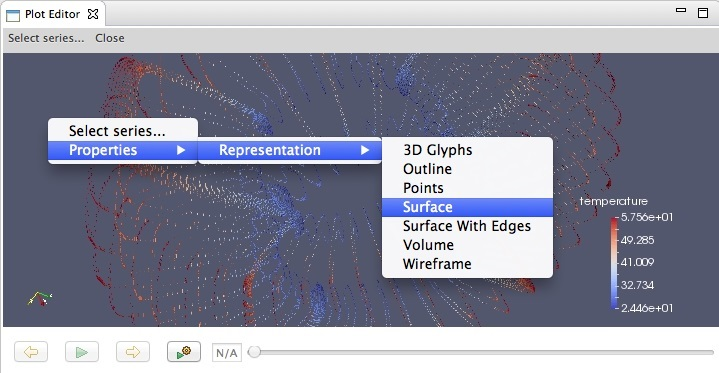
\includegraphics[width=12cm]{images/ParaViewRepresentationDropDown}
\end{center}

\subsubsection{Animation and Time Data}

The Plot Editor features a time slider widget at the bottom of the screen. 

\begin{center}
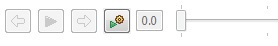
\includegraphics[width=12cm]{images/TimeSliderWidget}
\end{center}

The controls, in order of left to right, are:

1) Return to the previous time step.

2) Automatically play the plot as an animation by displaying the time steps
sequentially. 

3) Advance to the next time step. 

4) Opens an options menu that allows the user to set the playback speed, toggle
whether the animation should loop when it reaches the end, and set the plot to
the first or last time step.

5) A display for the current time step. It can be edited to set the plot to an
arbitrary time step. 

6) A slider that shows the current time step's position on the timeline. The
slider can be dragged around the timeline, setting the plot's time step
accordingly.

\section{Accessing a ParaView Web Server}

It is also possible to access the full ParaView web viewer application inside of
ICE. This allows for full access to all the web viewer's features.

\subsection{Accessing the Visualizer}

First, you must open a Plot Editor as described above.

\begin{center}
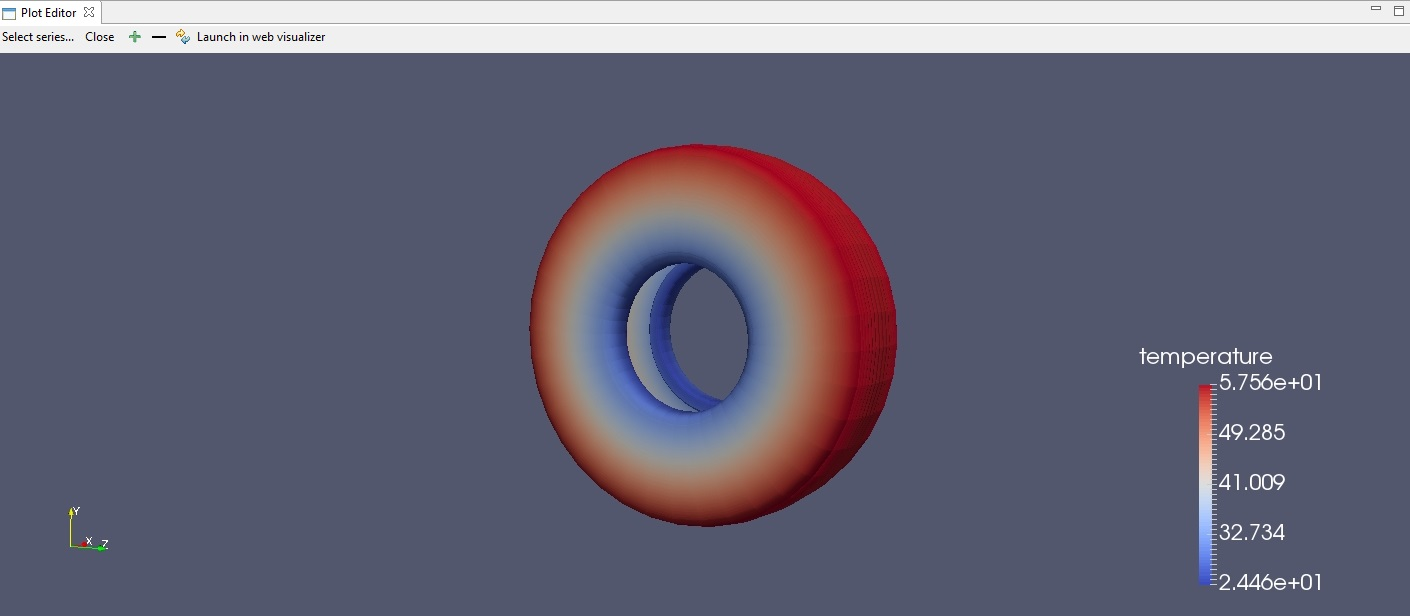
\includegraphics[width=12cm]{images/ParaViewPlotEditor}
\end{center}

Press the "Open in Web Visualizer" button in the top left to launch the web visualizer server and automatically open an internal web browser to view it.

\subsection{Using the Visualizer}

In order to load a data file, click the Show File List button as seen below.

\begin{center}
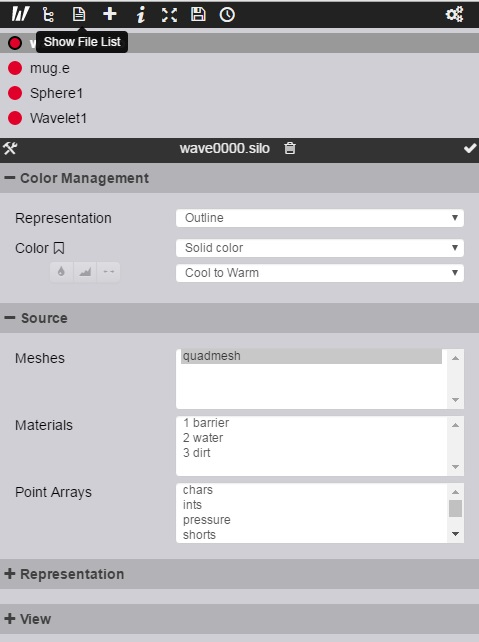
\includegraphics[width=12cm]{images/ParaViewVisualizer}
\end{center}

This will place the contents of the data directory into the side bar. For sessions, the data directory will be your ICE workspace. For a remote connection, this will be the folder containing the remote file you are visualizing. You may then double click on a file to load it into the model. 

You can click and drag the mouse to rotate the camera and right click followed
by dragging up or down to zoom. A full description of the visualizer's features
is beyond the scope of this tutorial, but see the official documentation
\href{http://www.paraview.org/ParaView3/Doc/Nightly/www/js-doc/index.html#!/guide/web_visualizer}{here}.

\graphicspath{{../../dynamicUI/src/}}
\chapter{Paraview}

ICE features functionality for visualizing models using ParaView.

\section{Installation and Configuration}

ParaView use for ICE requires a Mac OS or Linux operating system, as ICE does
not currently support ParaView connections on Windows. You will also need an
installation of ParaView on your local machine. ParaView can be downloaded from
its \href{http://www.paraview.org/download/}{official website}. The ICE
development team recommends using the latest available version of ParaView,
currently 5.0 at the time of this writing. You will further need a custom
Python HTTP web server implementation, which can be downloaded from the
\href{http://eclipseice.ornl.gov/downloads/paraview/scripts/http_pvw_server.py}{Oak
Ridge website}.

\subsection{Configuring the ParaView Connection}

Once ParaView is running, ICE must be configured to connect to the server. This
is done through specifying a default connection in the ICE Preferences page.
This process only needs to be performed once. After initially creating the
connection, ICE will attempt to connect to ParaView on that port each time it is
launched.

To set the connection, select Window $\rightarrow$ Preferences\ldots in ICE's
menu bar. (On Mac OS X, Preferences\ldots is located under ICE instead of
Windows.) Select Visualization $\rightarrow$ ParaView in the tree on the left
side of the Preferences window.

\begin{center}
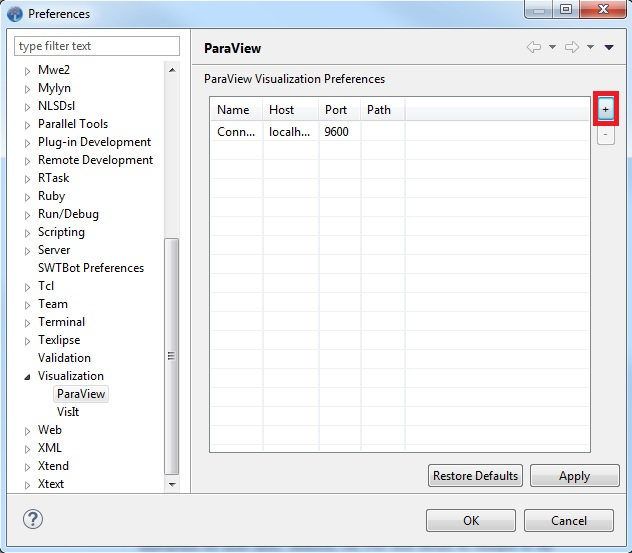
\includegraphics[width=12cm]{images/paraviewpreferencepage_ice}
\end{center}

Press the button with a ''+" symbol in the upper right (highlighted in the image
above) to add a new row to the table. Click on cells in the new row to edit
their values. 

\textbf{Name:} The connection's name. The default value will be fine.

\textbf{Host:} The hostname for the machine that will run ParaView. Use "localhost" if the machine running ICE will also be used to run ParaView.

\textbf{Port:} The port number on which the ParaView server will run. The default value will be fine, but if you change it, it must different from the Visualizer Port.

\textbf{Path:} The path to your ParaView installation. 

On Linux, the path will end with the top level folder into which ParaView was unzipped. For example, if you have a folder named ParaView on your desktop that contains the bin, doc, lib, and share folders, then your path would be /home/username/Desktop/ParaView. 

On Mac, the path will end with the folder containing your ParaView.app. For example, if you have installed ParaView to your Applications folder, the path will simply be /Applications

\textbf{Server Script Path:} The full path to the http_pvw_server.py file, ending with the folder containing it. For example if the file is on your desktop, the path might be /home/username/Desktop.

\textbf{Visualizer Port:} The port number for the ParaView web visualizer. The default value will be fine, but if you change it, then it must be different from the port number you provide for Port.

\textbf{Remote OS:} The operating system of the remote machine on which ParaView will be launched. If you want to launch ParaView on your local machine, ignore this cell. Otherwise, specify either "Linux" or "OSx".

\textbf{Remote ParaView Version Number:} The version of ParaView you are using. This may be ignored unless you are launching a remote ParaView session on a Linux machine. You can check your installation's version number by looking inside the top level \textbf{lib} folder. It will contain a folder named paraview- followed by the version number.

Once finished editing the cells in the new row, press Apply, then OK. ICE will
then launch the ParaView server and connect to it. If you are connecting to a remote machine, you will be prompted for permission to make the remote connection and asked for a password.

\section{Opening a ParaView File} 

To open a ParaView Plot Editor, a file that uses this editor must first be
placed in the Project Explorer. This view lists files imported into ICE. To
access the Project Explorer, use the the menu bar at the top of the window and
navigate to Window $\rightarrow$ Show View $\rightarrow$ Project Explorer.
Depending on the active Eclipse perspective, opening this view may require
selecting Other\ldots and finding the Project Explorer in the dialog under the
General category in the tree.

By default, the Project Explorer should automatically import the
ICEFiles/default and ICEFiles/itemDB folders. If it does not, or if you want to
import a different folder into ICE, right click in the Project Explorer and
select Import\ldots from the context menu. Then, select General $\rightarrow$
File System from the tree, and press the Next button. Select directories and/or
files to import into the Project Explorer, and enter which folder they should
be imported into, as shown below.

\begin{center}
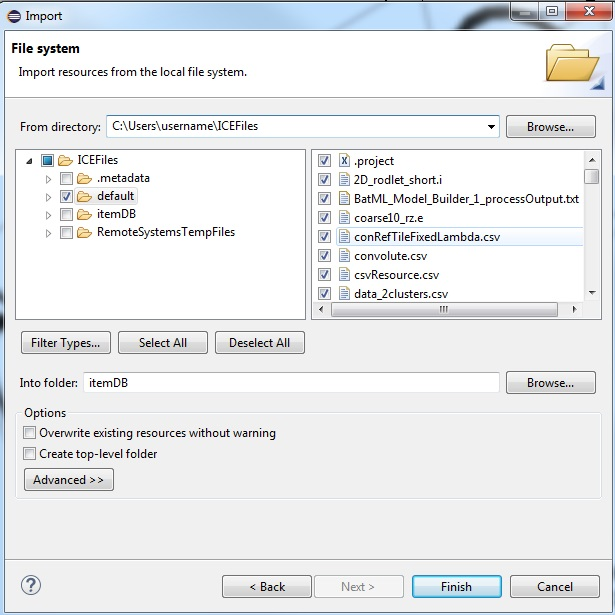
\includegraphics[width=12cm]{images/ImportFileDialog}
\end{center}

Once a file is in the Project Explorer, simply double click on it to open it in
ParaView. Local ParaView connections can only open local files, while remote ParaView connections can only open files on the remote host.

\subsection{Using ParaView}

\subsubsection{Camera Controls}

The Plot Editor allows the user to rotate the model by clicking and dragging
inside the display area or adjust the zoom by scrolling the mouse wheel.

\begin{center}
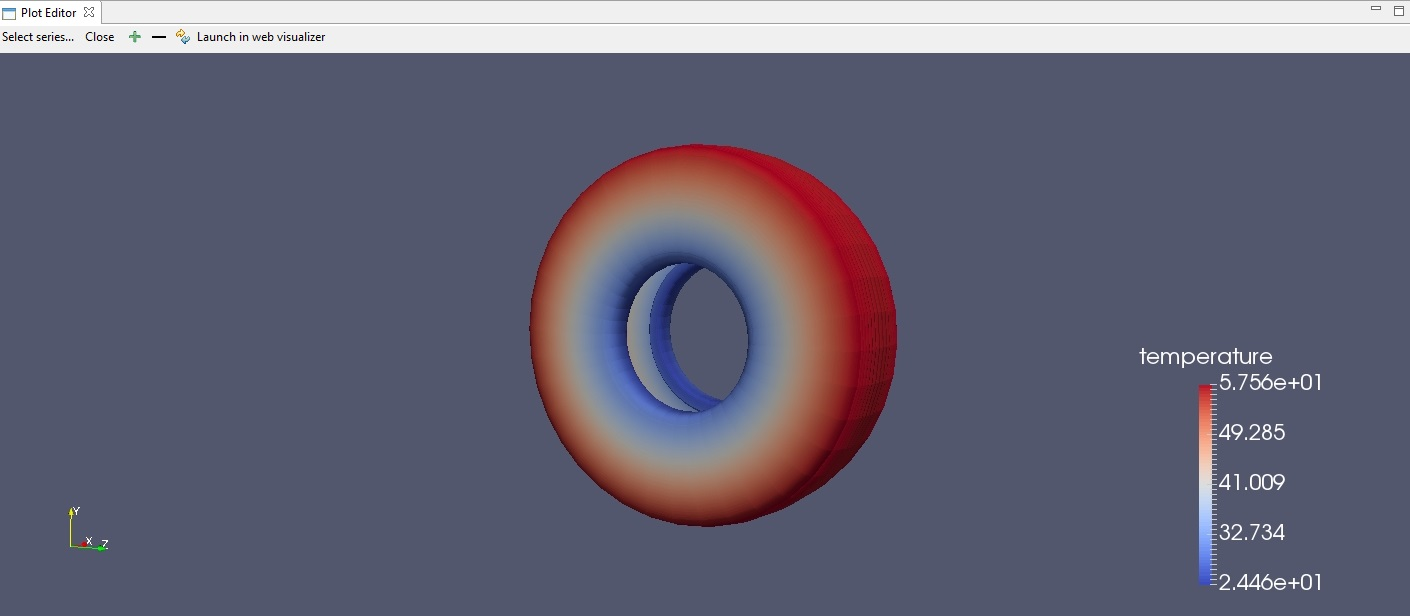
\includegraphics[width=12cm]{images/ParaViewPlotEditor}
\end{center}

The buttons in the upper left can also be used to manipulate the camera. The green plus sign will zoom in, while the black minus sign will zoom out. The green circular arrow button will reset the camera to its default position.

\subsubsection{Selecting the Plot}

Pressing the Select Series\ldots button will open a dialog which lists the
various plots in the opened file. Simply select one and click OK to open it. 

\begin{center}
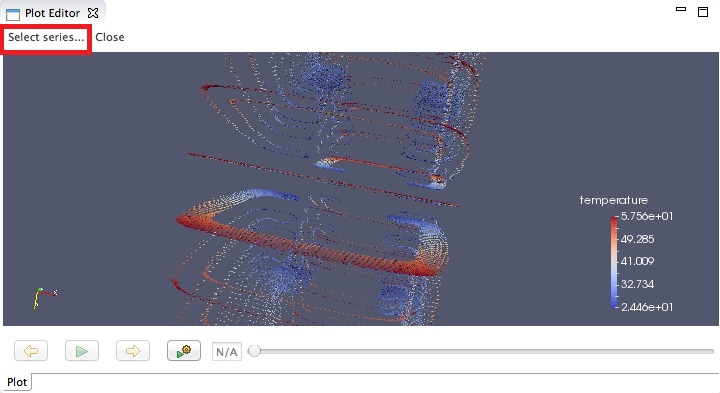
\includegraphics[width=12cm]{images/ParaViewPlotEditorSelectSeriesButton}
\end{center}

\subsubsection{Setting the Plot Representation} 

ParaView is capable of displaying plots in several different representations,
such as points or surfaces. To switch between plot type, right click inside the Plot
Editor's display area and select one of the listed options under the
Representation category in the context menu.

\begin{center}
\includegraphics[width=12cm]{images/ParaViewRepresentationDropDown}
\end{center}

\subsubsection{Animation and Time Data}

The Plot Editor features a time slider widget at the bottom of the screen. 

\begin{center}
\includegraphics[width=12cm]{images/TimeSliderWidget}
\end{center}

The controls, in order of left to right, are:

1) Return to the previous time step.

2) Automatically play the plot as an animation by displaying the time steps
sequentially. 

3) Advance to the next time step. 

4) Opens an options menu that allows the user to set the playback speed, toggle
whether the animation should loop when it reaches the end, and set the plot to
the first or last time step.

5) A display for the current time step. It can be edited to set the plot to an
arbitrary time step. 

6) A slider that shows the current time step's position on the timeline. The
slider can be dragged around the timeline, setting the plot's time step
accordingly.

\section{Accessing a ParaView Web Server}

It is also possible to access the full ParaView web viewer application inside of
ICE. This allows for full access to all the web viewer's features.

\subsection{Accessing the Visualizer}

First, you must open a Plot Editor as described above.

\begin{center}
\includegraphics[width=12cm]{images/ParaViewPlotEditor}
\end{center}

Press the "Open in Web Visualizer" button in the top left to launch the web visualizer server and automatically open an internal web browser to view it.

\subsection{Using the Visualizer}

In order to load a data file, click the Show File List button as seen below.

\begin{center}
\includegraphics[width=12cm]{images/ParaViewVisualizer}
\end{center}

This will place the contents of the data directory into the side bar. For sessions, the data directory will be your ICE workspace. For a remote connection, this will be the folder containing the remote file you are visualizing. You may then double click on a file to load it into the model. 

You can click and drag the mouse to rotate the camera and right click followed
by dragging up or down to zoom. A full description of the visualizer's features
is beyond the scope of this tutorial, but see the official documentation
\href{http://www.paraview.org/ParaView3/Doc/Nightly/www/js-doc/index.html#!/guide/web_visualizer}{here}.

\chapter{Wrap-Up}

\end{document}
